%====================================================================================================
% Controle PID
%====================================================================================================
% Plano de Trabalho
%----------------------------------------------------------------------------------------------------
% Autor			: Kelvim Rodrigues de Oliveira	
% Orientador		: Gedson Faria
% Instituição 		: UFMS - Universidade Federal do Mato Grosso do Sul
% Unidade		: CPCX - Campus de Coxim
%----------------------------------------------------------------------------------------------------
% Arquivo		: plano_trab_kelvim.tex
% Data de criação	: 13 de Maio de 2017
%====================================================================================================

\documentclass[a4paper,12pt,portuguese]{ufms-cpcx}

\usepackage[utf8]{inputenc}
\usepackage{amsmath,amssymb,latexsym}
\usepackage{float}
\usepackage{xcolor}
\usepackage{listings}
\usepackage[top=30mm,bottom=25mm,left=25mm,right=20mm]{geometry}
\usepackage{pdfpages}
\usepackage [onehalfspacing]{setspace} 
\usepackage{indentfirst}
%\usepackage{caption}
\usepackage[font=small]{caption}
\usepackage{subcaption}
\usepackage{multicol}
\usepackage{booktabs}	% http://ctan.org/pkg/booktabs
\usepackage{array}	% http://ctan.org/pkg/array
\usepackage[alf]{abntex2cite}


\newcolumntype{M}{>{\centering\arraybackslash}m{\dimexpr.25\linewidth-2\tabcolsep}}

\lstset{
	language=C++,
	basicstyle=\ttfamily\small, 
	keywordstyle=\color{blue}, 
	stringstyle=\color{verde}, 
	commentstyle=\color{red}, 
	extendedchars=true, 
	showspaces=false, 
	showstringspaces=false, 
	numbers=left,
	numberstyle=\tiny,
	breaklines=true, 
	backgroundcolor=\color{green!10},
	breakautoindent=true, 
	captionpos=b,
	xleftmargin=0pt,
}

\begin{document}
	% capa do trabalho %
\definecolor{verde}{rgb}{0,0.5,0}
\thispagestyle{empty}

\titulo{Trabalho de Conclusão de Curso\vskip 1.0cm
	Sistema embarcado para monitoramento e ajuste de velocidades de motores {CC} em robôs com duas rodas.}\vskip 0.5cm
\autor{Kelvim Rodrigues de Oliveira}

\orientacao{Prof. Dr. Gedson Faria}
%\docarea{Bacharelado em Sistemas de Informação}
\textofree{\large Bacharelado em Sistemas de Informação}

\vfill \centerline{
\includegraphics[scale=0.15]{figuras/ufms-logo.jpg}}

\vskip 0.5cm
\begin{center}
	Sistema de Informação\\
	Universidade Federal de Mato Grosso do Sul\\
	22 de dezembro de 2017
\end{center}

% contra capa %
\cleardoublepage
\thispagestyle{empty}
\begin{center}
	{\Large Sistema embarcado para monitoramento e ajuste de velocidades de motores {CC} em robôs com duas rodas.}
	
	\vspace{2cm}
	
	{\large\sc Kelvim Rodrigues de Oliveira.}
	
	\vspace{3cm}	
\end{center}

\hspace{5.5cm}
\begin{minipage}{10cm}
			{Orientador:\\Prof. Dr. Gedson Faria}\\
			
			\textit{Monografia apresentada como parte dos requisitos para obtenção do título de Bacharel em Sistemas de Informação do Câmpus de Coxim da UFMS.}
\end{minipage}	

\begin{center}
	\vspace{10cm}
	\textbf{Coxim - MS\\ 2017}	
\end{center}


\cleardoublepage
\thispagestyle{empty}
\vspace*{15cm}
Banca Examinadora:
\begin{itemize}
	\item Prof. Dr.  Gedson Faria (CPCX/UFMS) - Orientador
	\item Prof. Me.  Kleber Kruger (CPCX/UFMS) 
	\item Prof. Esp. Angelino Caon (IFMS--Coxim)
\end{itemize}

\chapter*{Agradecimentos}
\thispagestyle{empty}
Primeiramente a Deus por minha vida, família e amigos.

À instituição de ensino UFMS e ao campus de Coxim pelo ambiente criativo e amigável, pela paciência nos longos anos de formação.

Ao meu orientador Gedson e professores pela paciência e fé acreditando que este dia chegaria mesmo com muita demora.

Aos colegas que passaram as tardes na sala dos professores estudando e trocando conhecimentos.

Ao colega Rafael pelos conhecimentos a min transmitidos durante esse caminho.

Aos colegas da TalentW pelas inúmeras risadas e litros e litros de café.

A todos aqueles que direta ou indiretamente contribuirão para minha formação.

J.Rtf.
%Agradecer Orientador e Câmpus Coxim.

\chapter*{Resumo}
\thispagestyle{empty}
Robôs com duas rodas tem sido aplicado em diversas tipos de tarefas e também são os primeiros modelos de robôs carros estudados e implementados nos cursos de robótica devido a sua simplicidade quando comparado a robôs com quatro ou mais rodas. Estes modelos de robôs também são utilizados na competição de futebol de robôs da categoria VSS-RoboCup. Contudo, os robôs VSS da equipe Cedro/CPCX tiveram a dificuldade de movimentar-se em linha reta, pois por mais similares que sejam os motores de cada roda, o seu desempenho não é idêntico, tornando-se um grande problema pra equipe de futebol do Câmpus de Coxim.

Neste trabalho foi proposto um sistema embarcado que atua como uma ferramenta com sintaxe própria capaz de monitorar e determinar a diferença de velocidade entre os motores. 
Para esta finalidade, foram investigados dois modelos de controle, o controle do tipo PID (Proporcional, Integral e Derivativo), este controle faz correções sutis atingindo seu objetivo com maior suavidade. O segundo modelo, controle por pesos, consiste em um valor (peso) multiplicado pela potência solicitada torna o motor mais rápido equivalente ao mais lento.

Após investigado os controles do modelo PID verificou-se que o mesmo não seria eficiente para os jogadores de futebol visto que os controles desse tipo necessitam de informações de velocidade durante sua execução, informações estas obtidas utilizando-se de interrupções (ISR) a qual ocasiona erros de leitura tornando a ferramenta ineficaz.

Contornando os problemas de ISR, foi desenvolvido então um sistema embarcado, o qual utiliza-se das médias das contagens de interrupções para determinar a diferença relativa da velocidade entre os motores. Utilizando-se da sua sintaxe própria é possível tornar o sistema uma ferramenta capaz de testar, monitorar e ajustar regimes de potência. Utilizando um ou mais valores de PWM repetidos ou não conforme a estratégia empregada.

Por fim observou-se por meio dos testes, a necessidade dos ajustes em regimes de potências diferentes e que a ferramenta se mostrou eficaz como pré-ajuste do peso, para uma determinada velocidade, conforme a necessidade da competição.



\chapter*{Abstract}
\thispagestyle{empty}
Two-wheel robots have been used in many types of tasks and are also the first models of robot cars studied and implemented in robotics courses due to their simplicity when compared to robots with four or more wheels. These robot models are also used in the robot soccer competition of the VSS-RoboCup category. However, the VSS robots of the Cedro / CPCX team had the difficulty of moving in a straight line, because as similar as the motors of each wheel may be, their performance is not identical, becoming a big problem for Coxim's Campus soccer team.

In this paper, an embedded system that acts as a tool with its own syntax capable of monitoring and determining the speed difference between the motors was proposed .
For this purpose, two control models were investigated: the PID control (Proportional, Integral and Derivative); this control makes subtle corrections reaching its goal with greater smoothness. The second model, control by weight, consists of a value (weight) multiplied by the requested power that makes the faster motor equivalent to the slower one.

After investigating the controls of the PID model, it was verified that it would not be efficient for soccer players, since controls of this type need speed information during their execution, information obtained using interrupts (ISR) which cause read errors making the tool ineffective.

Bypassing the ISR problems, an embedded system was developed, which uses the average of the interrupt counts to determine the relative speed difference between the motors. By using its own syntax it is possible to make the system a tool capable of testing, monitoring and adjusting power regimes, using one or more PWM values, repeated or not, according to the strategy employed.

Finally, it was observed through the tests, the need for adjustments in different power regimes and that the tool proved to be effective as a pre-adjustment of the weight, for a certain speed, according to the need of the competition.


% sumario %
\cleardoublepage
\pagenumbering{roman}
\setcounter{page}{1}
\tableofcontents

% lista figuras %
\cleardoublepage
\addcontentsline{toc}{chapter}{Lista de Figuras}
\listoffigures

% lista tabelas%
\cleardoublepage
\addcontentsline{toc}{chapter}{Lista de Tabelas}
\listoftables

\cleardoublepage
\pagenumbering{arabic}
\setcounter{page}{1}

\chapter{Introdução}
Os carros os quais estamos acostumados possuem quatro rodas e dois eixos, o eixo dianteiro é responsável pelas manobras virando as rodas R1 e R3 (Figura~\ref{fig:carrocurva}) em sua extremidade mudando a direção do movimento conforme D1 e D3 (Figura~\ref{fig:carrocurva}).
\begin{figure}[H]
	\centering
	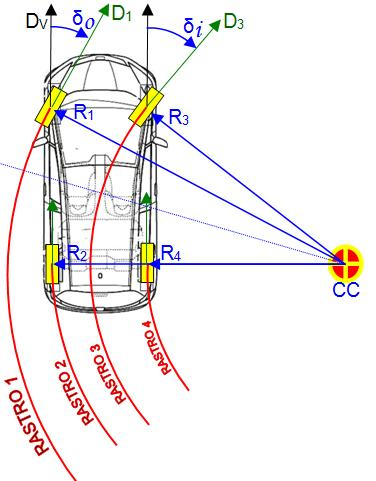
\includegraphics[width=0.5\textwidth]{Curva.jpg}
	\caption{Mecânica dos movimentos. Fonte: www.ebanataw.com.br}
	\label{fig:carrocurva}
\end{figure}
Diferente dos carros de quatro rodas, o robô Modu nome dado ao robô jogador de futebol membro da equipe de futebol de robôs do Câmpus de Coxim, doado por Carlos Eduardo Rodrigues e Paulo Vinícius Santos, se move similar aos tanques de guerra, que possuem duas fontes de tração independentes para realizar os movimentos e suas manobras.
Com dois conjuntos roda-motor independentes, o Modu ativa seus motores em sentidos opostos para realizar o movimento de rotação em seu próprio eixo, emprega potências diferentes e sentidos iguais para realizar curvas e emprega potências iguais para ir em linha reta. 

Porém, o movimento retilíneo se tornou um desafio para equipe de do Câmpus de Coxim, pois mesmo com motores idênticos em marca, potência e modelo, estes apresentam diferenças em sua velocidade de rotação, realizando o movimento de curva, mesmo com os motores recebendo a mesma tensão. Apesar das influências externas não serem uma constante estas influencias se mostram tendenciosa para um lado.

 % como pode ser visto no gráfico abaixo, a relação da proporção da velocidade do motor A em relação a velocidade do motor B em percentagem \%
%\begin{figure}[H]	
% 	\centering
% 	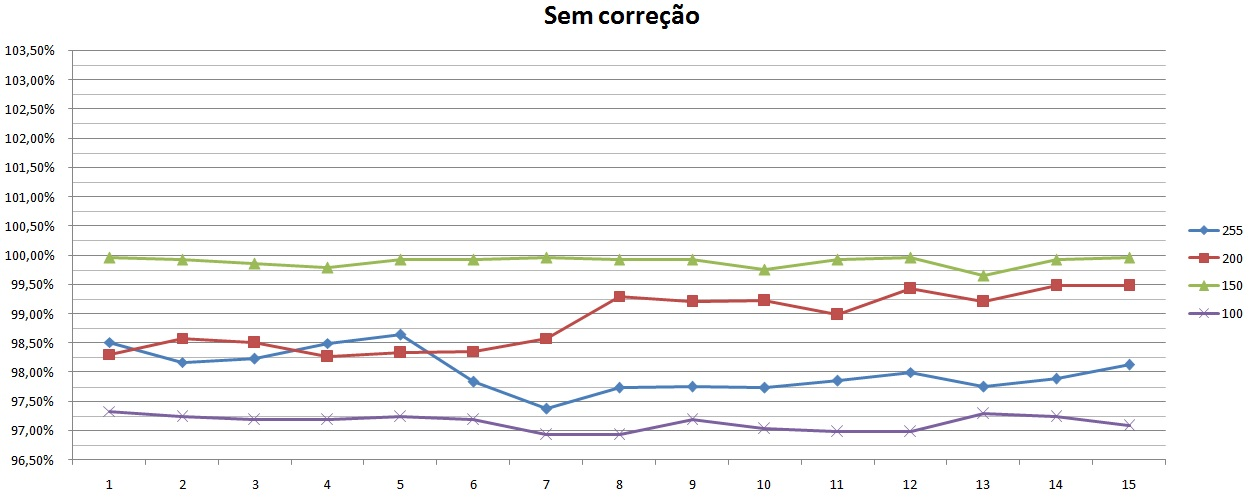
\includegraphics[width=1\textwidth]{semcorrecao.jpg}
% 	\caption{Velocidades do motor A em relação ao motor B em \%, quinze comparações para cada valor de PWM. Valores de PWM testados: 100, 150, 200 e 255}
% \end{figure}

 Devido a este problema foi então desenvolvido uma ferramenta a qual permite realizar o estudo das diferenças entre os motores em diferentes regimes de potência, com uma sintaxe própria e de fácil utilização pode-se achar o peso (valor de ajuste) o qual aplicado nos valores de PWM selecionados trás uma equidade quanto a velocidade das rodas, adequado-se conforme a necessidade de cada equipe.

 \section{Objetivos}
 
 
 \subsection*{Objetivo Geral} 
  
 O objetivo principal deste trabalho é estudar e implementar uma ferramenta capaz de monitorar a odometria de cada uma das rodas em diferentes regimes de potência. 
 %um peso afim de compensar o excedente de potência do motor mais rápido trazendo igualdade de velocidade entre os motores esquerdo e direito do robô. 

\subsection*{Objetivos Específicos}

\begin{itemize}
	%lista de itens	
	
	\item Estudar o hardware do Arduino com foco em PWM e interrupções.
	\item Desenvolver software embarcado utilizando a linguagem C para IDE do Arduino.
	\item Realizar um estudo com o objetivo de tornar o robô MODU mais funcional para o time de futebol do CPCX.
	
\end{itemize}

\section {Organização da Monografia}
No Capítulo 2 é apresentado ambiente do futebol de robôs e suas modalidades.
No Capítulo 3 estão descritos os detalhes dos componentes eletrônicos e chassis do robô Modu.
No Capítulo 4 tem-se tutoriais para instalação das IDEs: Arduino IDE e Clion, e também do PlarformIO.
O estudo das interrupções no Atmega328 é apresentado no Capítulo 5.
No Capítulo 6 descreve-se a teoria do modelo PID e os problemas de sua implementação no Atmega328. Ainda no Capítulo 6, são descritas as características de implementação da ferramenta de monitoramento e ajuste de velocidades, bem como os testes de calibração dos motores.
No Capítulo 7 faz-se uma discussão dos resultados obtidos pela utilização da ferramenta com PWMs de 100, 150, 200 e 255.
Por fim, no Capítulo 8, são apresentadas as considerações finais, as principais contribuições e sugestões para trabalhos futuros.


\chapter{Futebol de robôs}
%Este capitulo destina-se alguns conceitos, informações e história do futebol de robôs, suas principais modalidades, dinâmica de jogo e movimentos.
%

\section{Uma breve história sobre futebol de robôs}
A FIRA, sigla em inglês para \textit{Federation of International Robot-soccer Association} e a RoboCup associações, duas organizações de referência mundial para o estudo e organização quanto ao futebol de robôs, que tem como objetivo promover pesquisas nas áreas de robótica e inteligência artificial, estimulando o interesse dos participantes a resolver problemas. 

A FIRA, fundada no ano de 1995 pelo professor Kim Jong-Hwan, realizou seu primeiro campeonato mundial na Coréia em 1997, dois anos após sua fundação, com o objetivo de levar aos leigos e as gerações jovens o espírito da ciência e tecnologia aplicada à robótica. Desde então, a FIRA vem realizando diversos eventos em vários países do mundo, incluindo o Brasil, o que fez com que o futebol de robôs obtivesse reconhecimento mundial. O Brasil, teve a oportunidade de sediar a Copa do Mundo em agosto de 1999, realizada entre os dias 4 a 8, na cidade Campinas no estado de São Paulo.

A RoboCup foi criada no Japão por meio da iniciativa de um grupo de pesquisadores que tinham como objetivo em comum, o jogo de futebol com a finalidade de promover o crescimento da ciência e tecnologia. De forma independente, os professores Minoru Asada da Universidade de Osaka, e a Professora Manuela Veloso junto a seu aluno Peter Stone da Universidade Carnegie Mellon, EUA, estavam também trabalhando em robôs jogadores de futebol.
O primeiro campeonato da Robocup junto a primeira conferência, foi realizados em 1997, onde compareceram mais de 40 equipes e mais de 5.000 espectadores. Infelizmente no Brasil, até o momento, não foram realizados eventos da Robocup com âmbito mundial~\cite{lourivaljr}.

\section{Modalidade} \label{modalidade}
Assim como o futebol jogado por humanos, o futebol de robôs também tem suas regras de jogo bem definidas. A FIRA Cup é um evento organizado com competições de várias categorias, destacam-se as categorias \textit{Micro-Robot Soccer Tournament} (MiroSot) e a \textit{Humanoid Robot Soccer Tournament} (HuroSot), ambas são disputadas sob o olhar de um árbitro humano, já a categoria \textit{Simulated Robot Soccer Tournament} (SimuroSot), que como o próprio nome sugere, trata-se de uma modalidade de simulação, quando não se tem a disposição os recursos de hardware referentes aos robôs.

Na categoria \textbf{VSS} do inglês \textit{\textbf{IEEE Very Small Size}} a competição ocorre durante a RoboCup, a versão sul-americana da competição, cuja categoria é voltada para partidas com pequenos robôs que se movimentam através de dois motor, um motor para cada roda, realizando movimentos rápidos, os robôs são controlados remotamente, mas sem intervenção humana, os comandos são enviados a partir de um computador disposto com uma inteligência artificial e suas estratégias. Está inteligência por sua vez utiliza-se do processamento das imagens de vídeo das câmeras dispostas em cima do campo. Sendo este o ambiente principal do trabalho.
A partida deve ser jogada por duas equipes, com três robôs cada, um robô pode atuar como goleiro de acordo com as estratégias, já fora de campo o time contem três membros humanos, o ``gerente", o ``técnico" e um ``instrutor" os quais só tem acesso ao palco. Cada equipe possui seu computador o qual é principalmente dedicado ao processamento de visão, identificação e de localização.  
O tamanho dos robôs desta categoria é limitado a 7,5 cm x 7,5 cm x 7,5 cm, altura da antena não deve ser considerada na medição do tamanho de um robô. É utilizado uma bola de golfe de cor laranja com intuito de facilitar o processo de visão computacional~\cite{sane}.
Esta categoria conta com duas ligas, a ``\textit{Large league}" (Liga grande) considerado grande pois o seu campo possui as dimensões de 400cm x 280cm e a ``\textit{Middle league}" (Liga média) que tem seu campo menor com as dimensões de 220cm x 180cm.

\chapter{O robô Modu}
O time de futebol de robôs do Câmpus de Coxim enquadra-se na modalidade VSS conforme a seção \ref{modalidade} e, portanto, está limitado às dimensões de 7,5 cm x 7,5 cm x 7,5 cm. Dotado de um Arduino Nano o qual realiza o controle de todo o robô, um bluetooth do modelo \textbf{HC-06} (Seção~\ref{bthc06}) que possui apenas o modo \textit{slave} (apenas recebe conexão, não busca a mesma) cuja função principal é estabelecer a conexão entre o robô e o computador ``técnico" da equipe, um driver para motor de corrente contínua do modelo \textbf{TB6612FNG}~(Seção~\ref{TB6612FNG}) capaz de controlar dois motores, dos quais são utilizados para realizar os movimentos, dois sensores ópticos do modelo \textbf{TCRT1000} (Seção~\ref{TCRT1000}) os quais são utilizados em conjunto com as rodas (Seção~\ref{roda}), e este conjunto trabalha como um encoder, utilizado para determinar a velocidade de rotação das rodas/motor.
\begin{figure}[H]
	\centering
	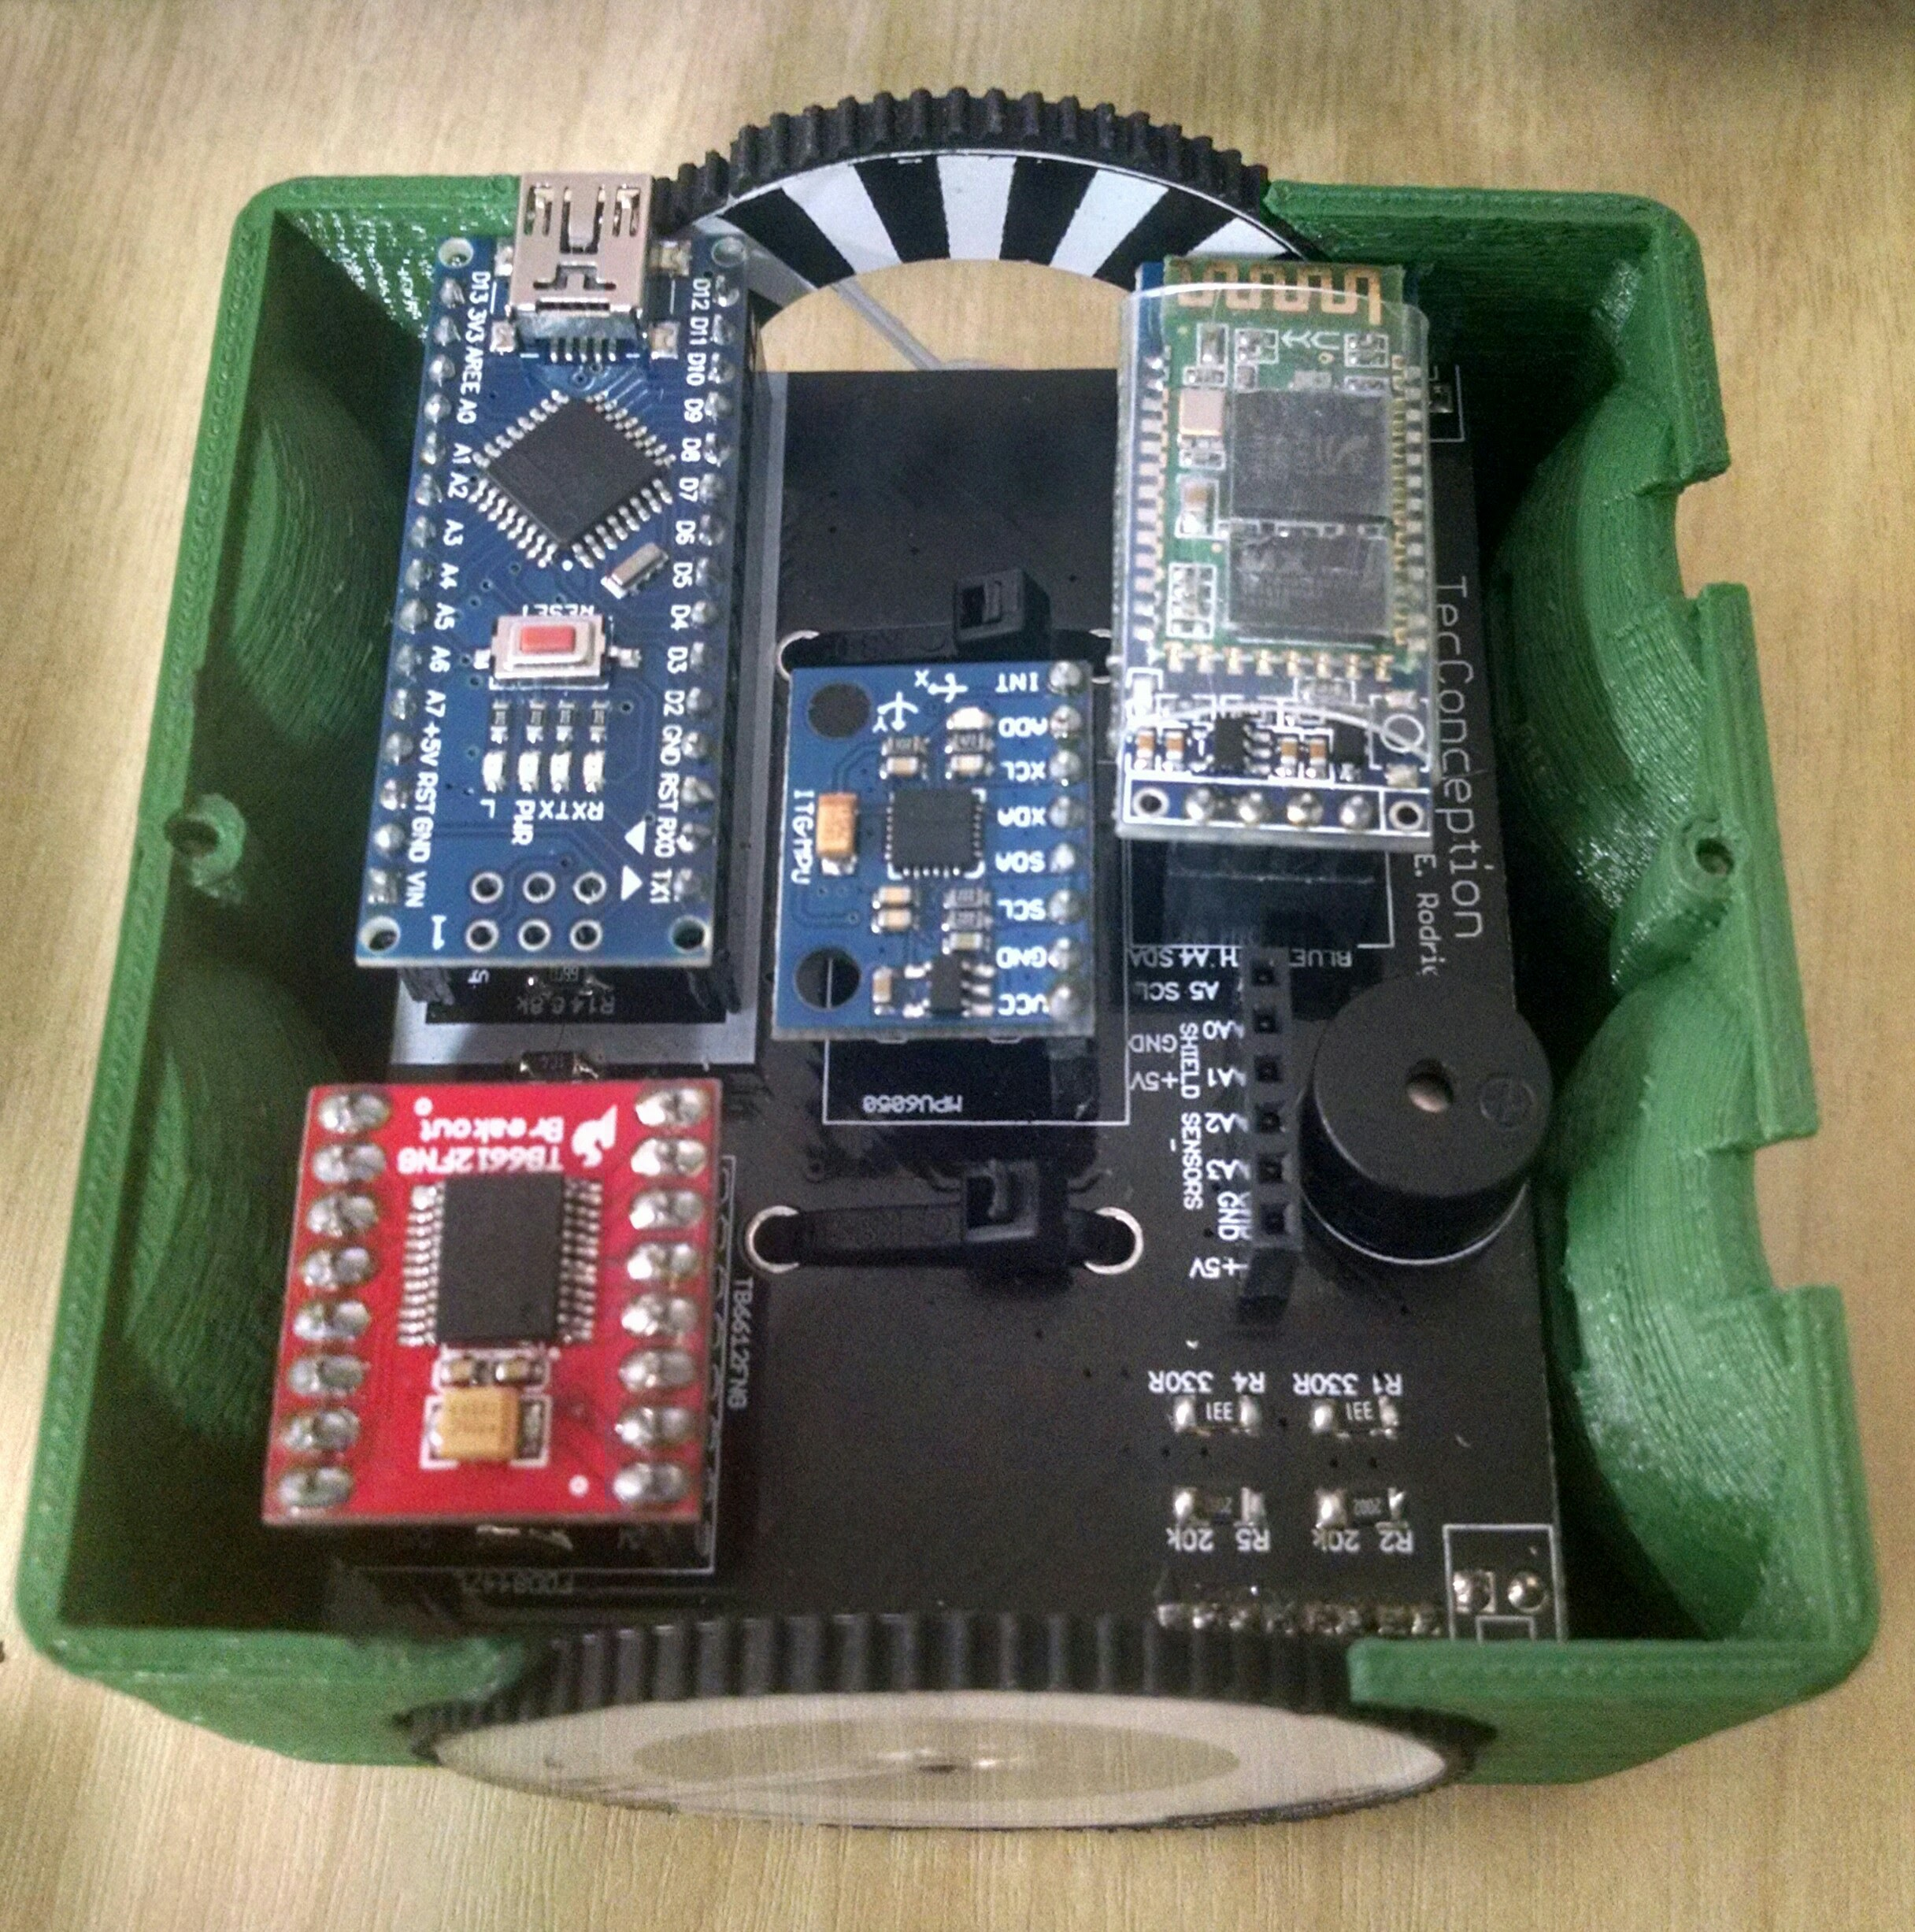
\includegraphics[width=0.5\textwidth]{superiormodu.jpg}
	\caption{Vista superior do robô Modu.}
\end{figure}
\begin{figure}[H]
	\centering
	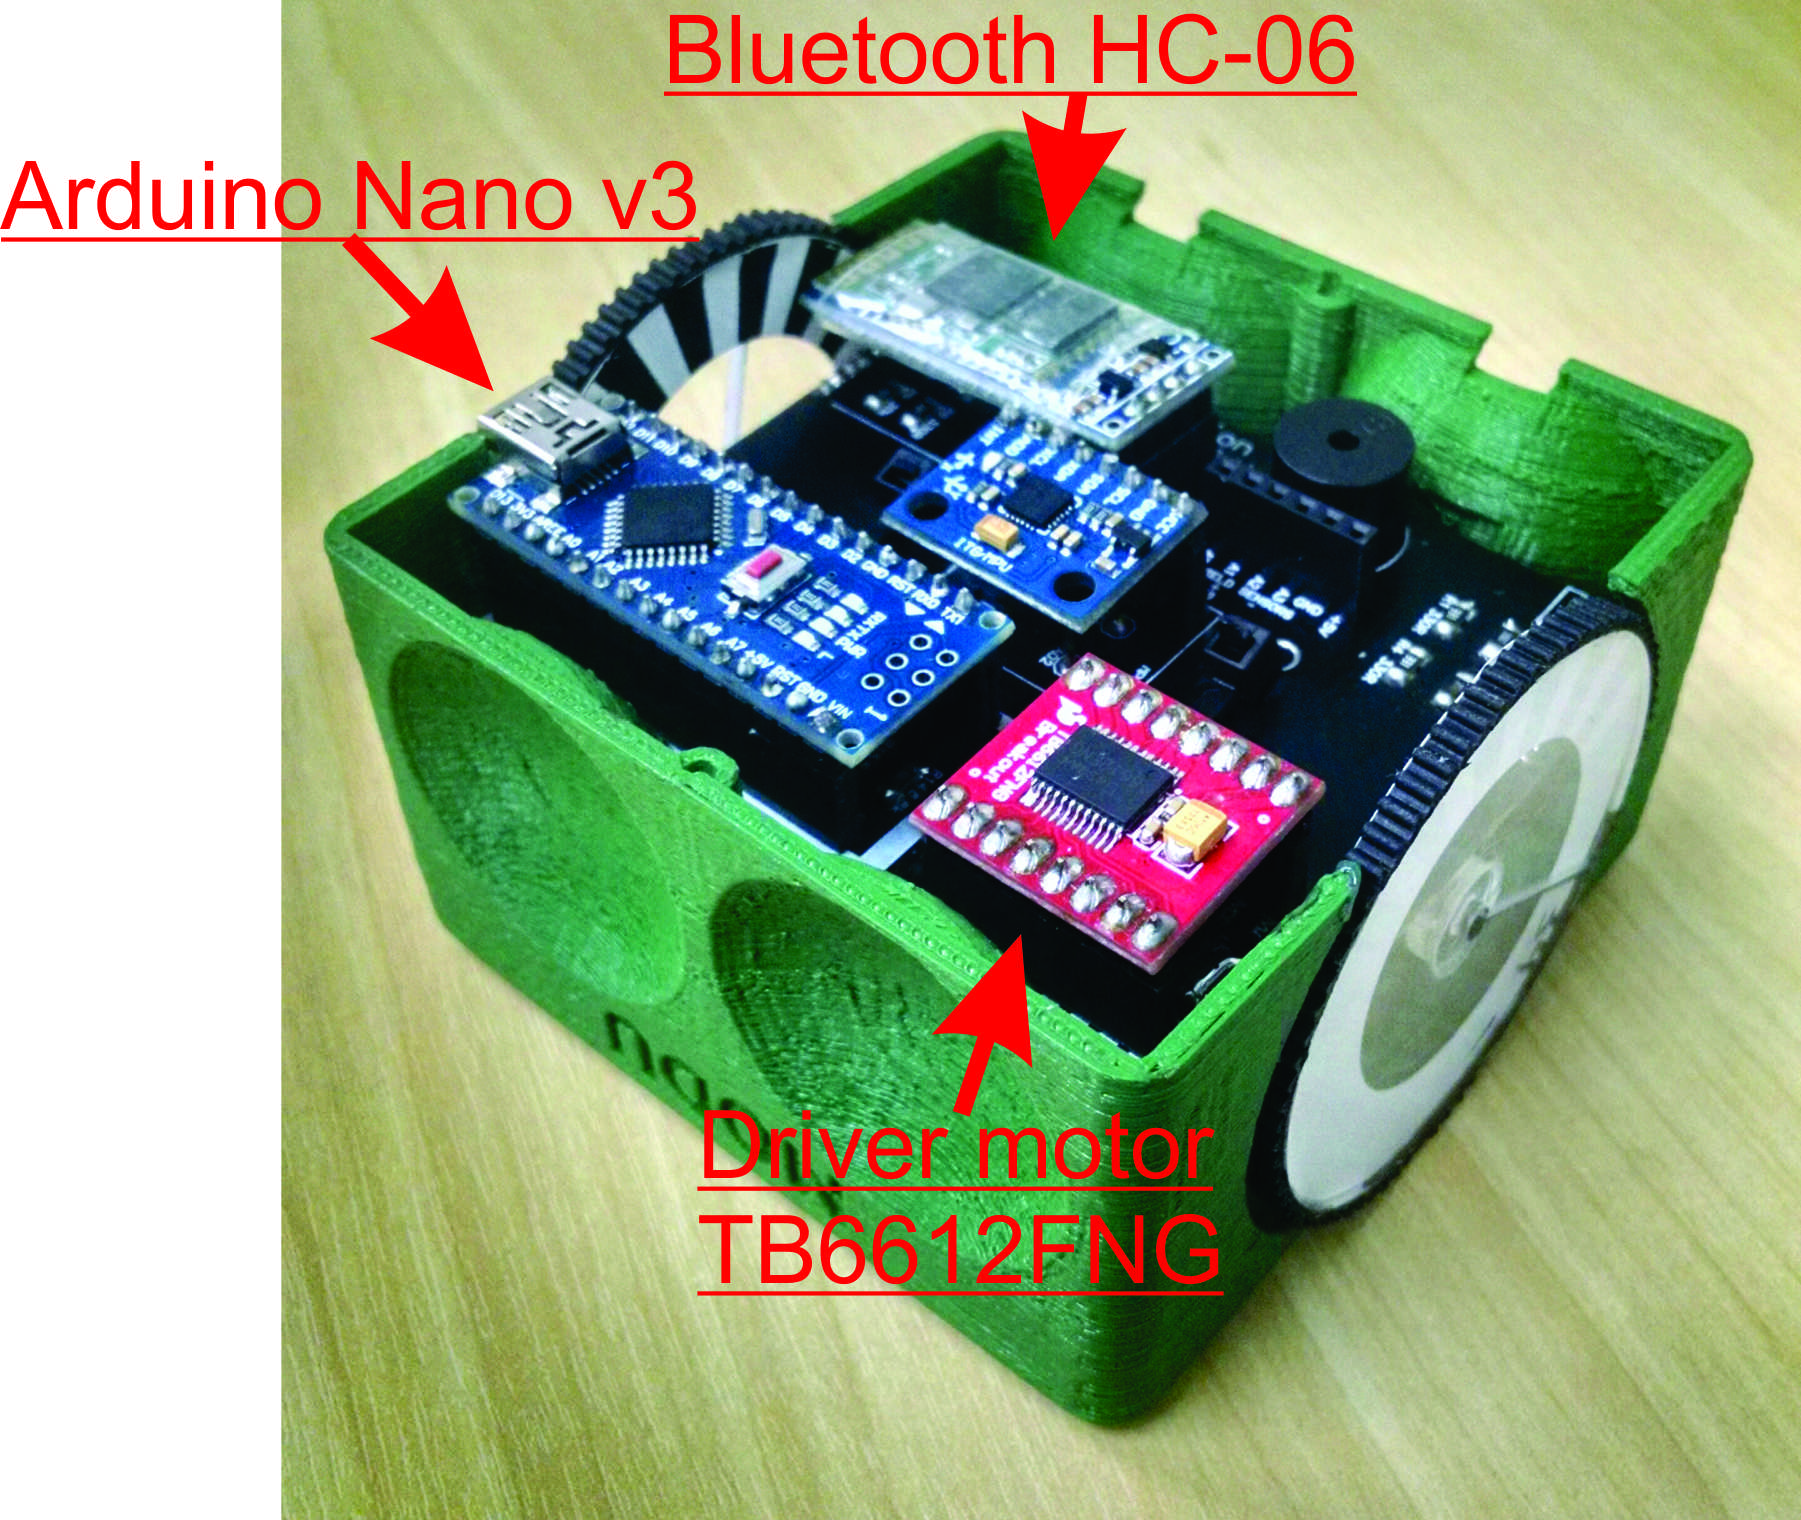
\includegraphics[width=0.5\textwidth]{inferiormodu.jpg}
	\caption{Vista inferior aberto do robô Modu.}
\end{figure}


\section{Arduino}\label{arduinonano}
Todas as versões do Arduino são baseadas em um microprocessador Atmel AVR de 8 bits de arquitetura RISC~\cite{arduinoemacao}. O Arduino Nano versão 3.0 utilizado no robô Modu (Figura~\ref{fig:arduinonano}), possui um processador ATmega328 provido de uma memória flash de 32 KB no total, sendo 2 KB utilizados pelo \textit{bootloader} deixando disponível 30 KB, com uma velocidade de clock de 16 MHz. Contém uma porta mini-USB integrada que serve para troca de dados e também como fornecimento de energia. 
\begin{figure}[H]
	\centering
	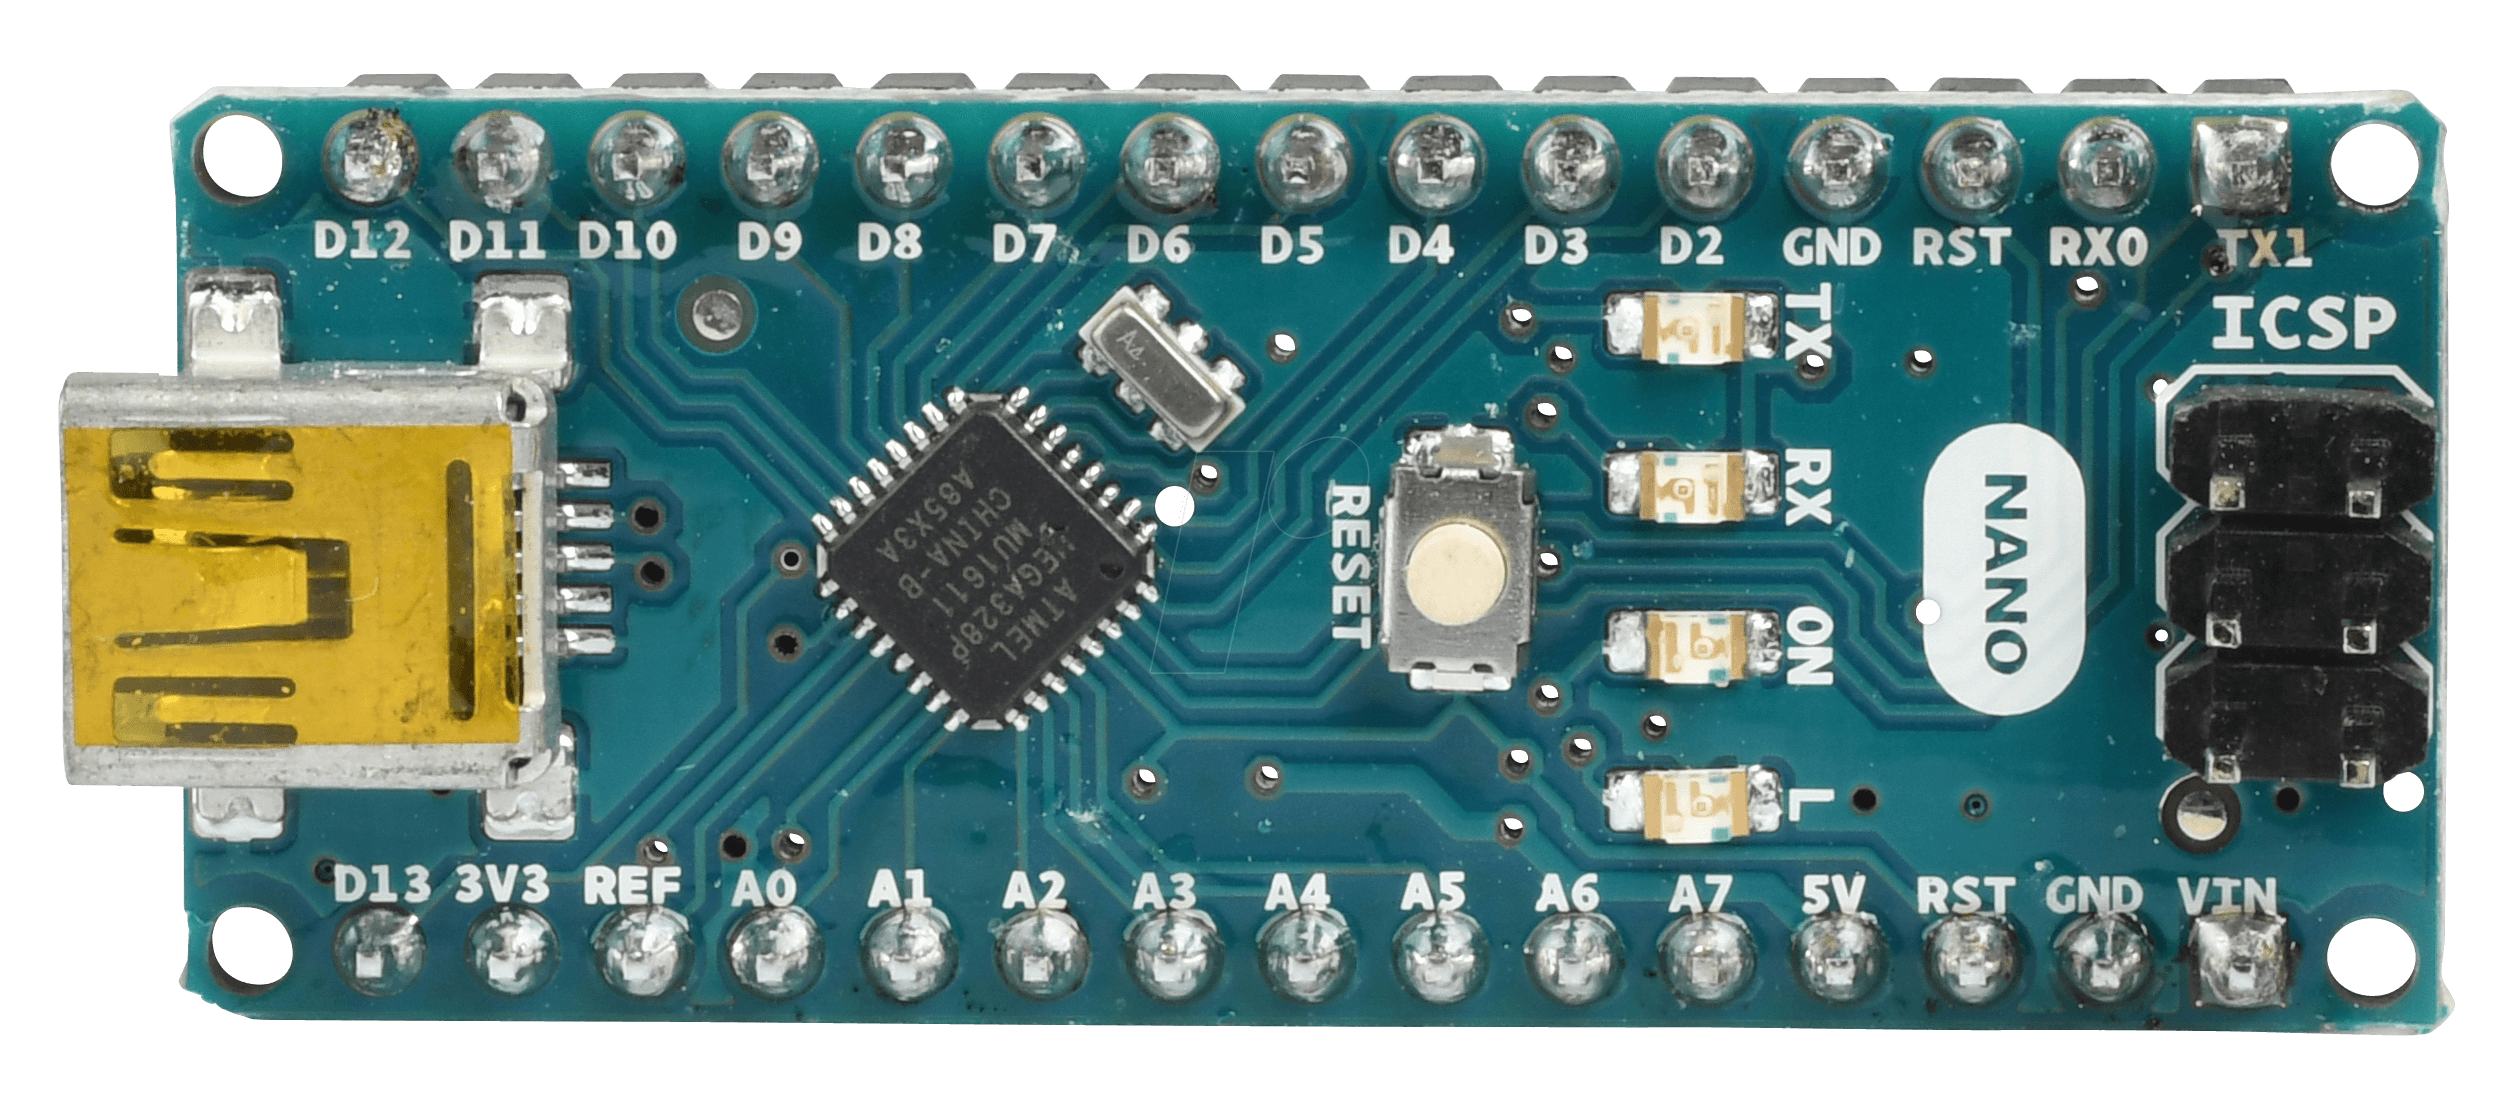
\includegraphics[width=0.5\textwidth]{arduinonano.png}
	\caption{Vista superior de um Arduino Nano. Fonte: http://store.arduino.cc}
	\label{fig:arduinonano}
\end{figure}
O Arduino Nano tem a opção de receber energia também pelo pino 30 (VIN) em tensões de 6 a 20 volts e/ou pelo pino 27 (5V) uma tensão regulada de 5,5 volts, caso estejam as três fontes de energias conectadas a placa seleciona a de maior tensão para seu funcionamento. Dotado também de uma comunicação serial que possibilita o Arduino se comunicar com um computador ou com outros dispositivos, como o bluetooth neste projeto, o Arduino Nano possui uma porta serial, também chamada UART ou USART, são acessadas pelos pinos digitais 0 (RX) e 1 (TX), assim como uma conexão USB, por isso é necessário um driver serial para utilizá-lo junto ao computador. Sendo assim, quando se usa esta funcionalidade, os pinos 0 e 1 não poderão ser utilizados como entrada ou saída digital. A localização destes pinos, bem como as funções dos demais pinos do Arduino Nano podem ser vistas na Figura~\ref{fig:pinagem}.
\begin{figure}[H]
	\centering
	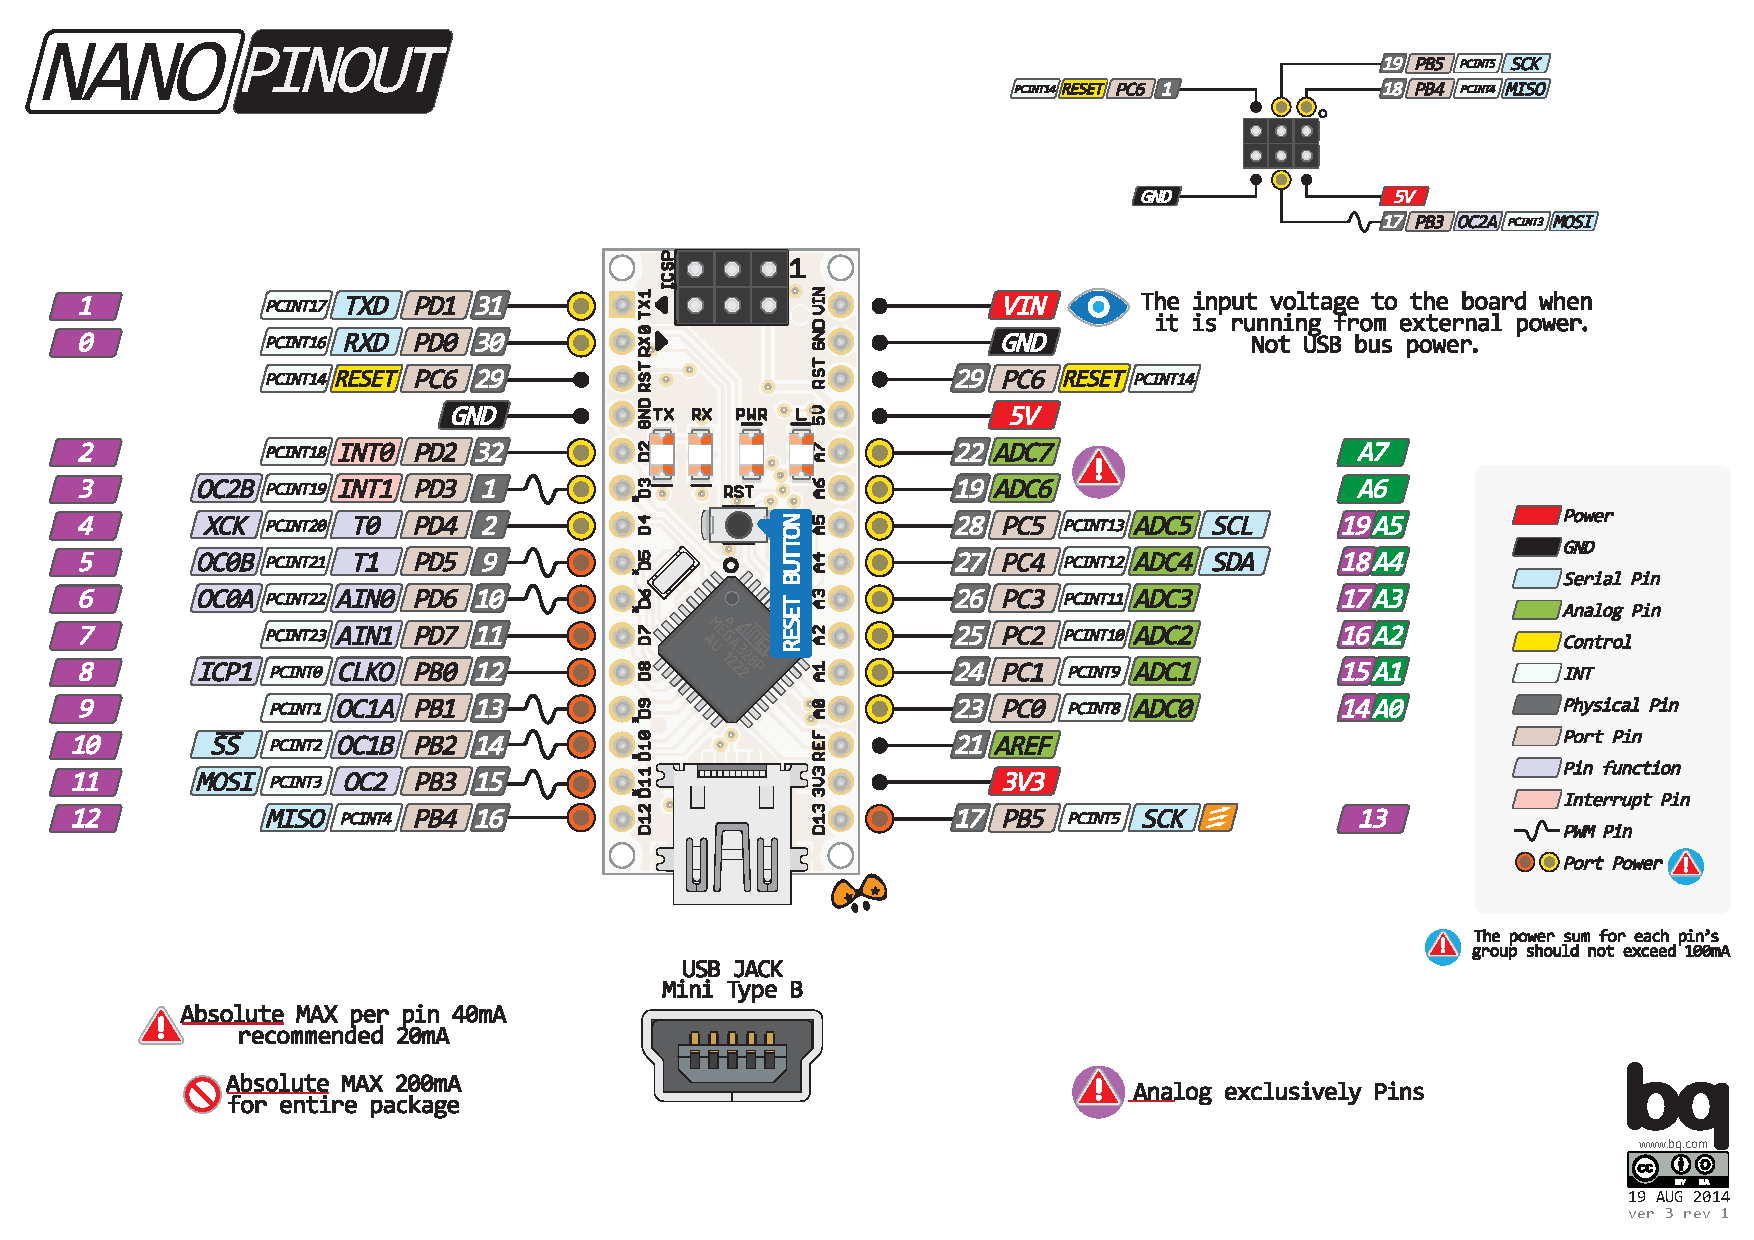
\includegraphics[width=0.9\textwidth]{nano.pdf}
	\caption{Infográfico pinagem arduino e suas funções}
	\label{fig:pinagem}
\end{figure}
Na IDE do Arduino existe uma ferramenta que disponibiliza o monitoramento da comunicação Serial entre o Arduino Nano e o computador. O Arduino Nano, trata-se de um componente de grande utilidade, capacidade, e de pequenas dimensões (18 mm x 45 mm) e pesando apenas 7 gramas o tornam ideal para um robô jogador de futebol. 


\section{Driver TB6612FNG para motores CC}\label{TB6612FNG}
Segundo o \textit{datasheet} disponibilizado pela empresa Toshiba, o \textbf{TB6612FNG} é um driver que pode controlar até dois motores de corrente contínua (CC), designados como A e B. Com o total de 16 pinos, dois pinos de entrada definem o sentido de rotação do motor, sendo \textbf{AIN1,AIN2} controlando o sentido do motor A e \textbf{BIN1,BIN2} para o motor B. Dois pinos de saída, conectados diretamente no motor, \textbf{A01, A02} e \textbf{B01 e B02} para os motores A e B respectivamente. A velocidade de cada motor pode ser controlada por um sinal de \textbf{PWM} nos seus respectivos pinos \textbf{PWMA} e \textbf{PWMB}, o driver possui um pino \textbf{STBY}, abreviação do inglês \textit{standby} que pode ser traduzido para espera, ou seja, modo de espera, para retira-lo do modo de espera deve-se colocar a tensão deste pino em alta (\textit{HIGH}). O pino \textbf{VCC} é destinado a suprir a demanda de energia do circuito, sendo operacional com tensões de 2,7 até 5,5 volts de corrente contínua, já o pino \textbf{VM} é destinado a suprir a demanda de energia dos motores, tendo seu limite máximo de 15 volts em corrente contínua. 

\begin{figure}[H]
	\centering
	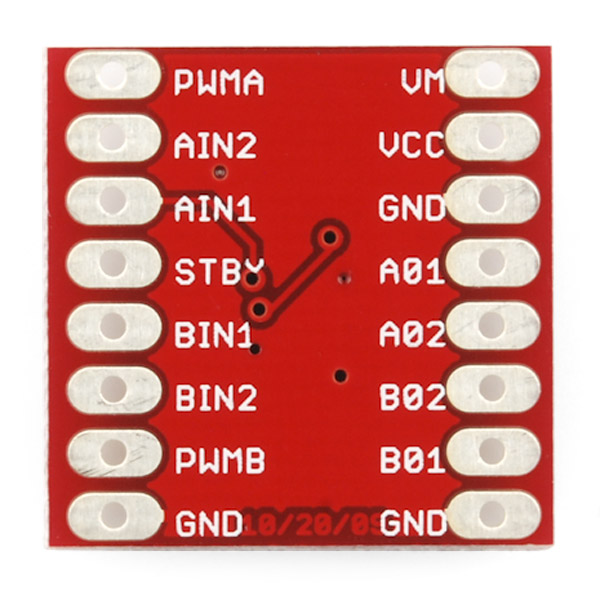
\includegraphics[width=0.5\textwidth]{inferiorTB6612FNG.jpg}
	\caption{Vista inferior do driver TB6612FNG com os rótulos de seus respectivos pinos. Fonte: http://www.sparkfun.com}
\end{figure}

Para entendermos o funcionamento básico do controlador \textbf{TB6612FNG} a tabela a seguir descreve as possibilidades de configuração para o controlador, considerando que o pino \textit{\textbf{STBY}} e \textit{\textbf{PWM}} estão em alto(\textit{high}) em todos os casos, ou seja, os casos de \textit{\textbf{STBY/PWM}} baixos(\textit{low}) não estarão presentes na tabela.
\begin{table}[!h]
	\renewcommand{\arraystretch}{1.3}
	\centering
	\begin{tabular}{|c|c|c|c|c|}
		\hline
		\textbf{IN1} & \textbf{IN2} & \textbf{OUT1} & \textbf{OUT2} & \textbf{MODO} \\ \hline
		    ALTO     &     ALTO     &     BAIXO     &     BAIXO     & FREADA RÁPIDA \\ \hline
		   BAIXO     &     ALTO     &     BAIXO     &     ALTO      &   ROTAÇÃO 1   \\ \hline
		    ALTO     &    BAIXO     &     ALTO      &     BAIXO     &   ROTAÇÃO 2   \\ \hline
		   BAIXO     &    BAIXO     &   DESLIGADO   &   DESLIGADO   &    PARADO     \\ \hline
	\end{tabular}
	\caption[Tabela verdade controle motor]{Lista de funcionamento e atuação de um motor CC para o controlador TB6612FNG.}
	\label{Tab:TB6612FNG}
\end{table}

Como pode ser visto na Tabela~\ref{Tab:TB6612FNG} com as duas entradas (IN1 e IN2) ALTO não há corrente de saída em ambas as saídas, alternando a corrente entre as portas \textbf{IN1} e \textbf{IN2} mudamos o sentido de rotação do motor e por último com as duas entradas sem carga as portas \textbf{OUT} não apresentam saída de tensão, sendo assim controlando as portas \textbf{IN} com o Arduino podemos controlar o sentido de rotação de cada um dos motores, visto que o \textbf{TB6612FNG} pode controlar até dois motores.

\section{Sensor Óptico TCRT1000}\label{TCRT1000}
O sensor óptico do modelo \textbf{TCRT1000}, segundo a documentação da empresa \textit{\textbf{Vishay}} obtidas no site \textit{www.vishay.com}, é um conjunto, contendo um emissor infravermelho ao lado de um fototransistor, como pode ser vistos na Figura~\ref{fig:TCRT1000}. 
\begin{figure}[H]
	\centering
	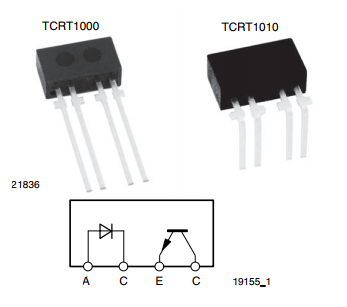
\includegraphics[width=0.4\textwidth]{TCRT1000.jpg}
	\caption{Sensor óptico TCRT1000. Fonte:www.vishay.com}
	\label{fig:TCRT1000}
\end{figure}
Inseridos em um invólucro de chumbo capaz de bloquear a luz visível, evitando erros de leitura pelo fototransistor. Um sensor de pequenas dimensões medindo 7mm x 4mm x 2,5mm e pode ser utilizado como um sensor de odometria em robô com dois sensores para cada roda (Figura~\ref{fig:lateralmodu}).
\begin{figure}[H]
	\centering
	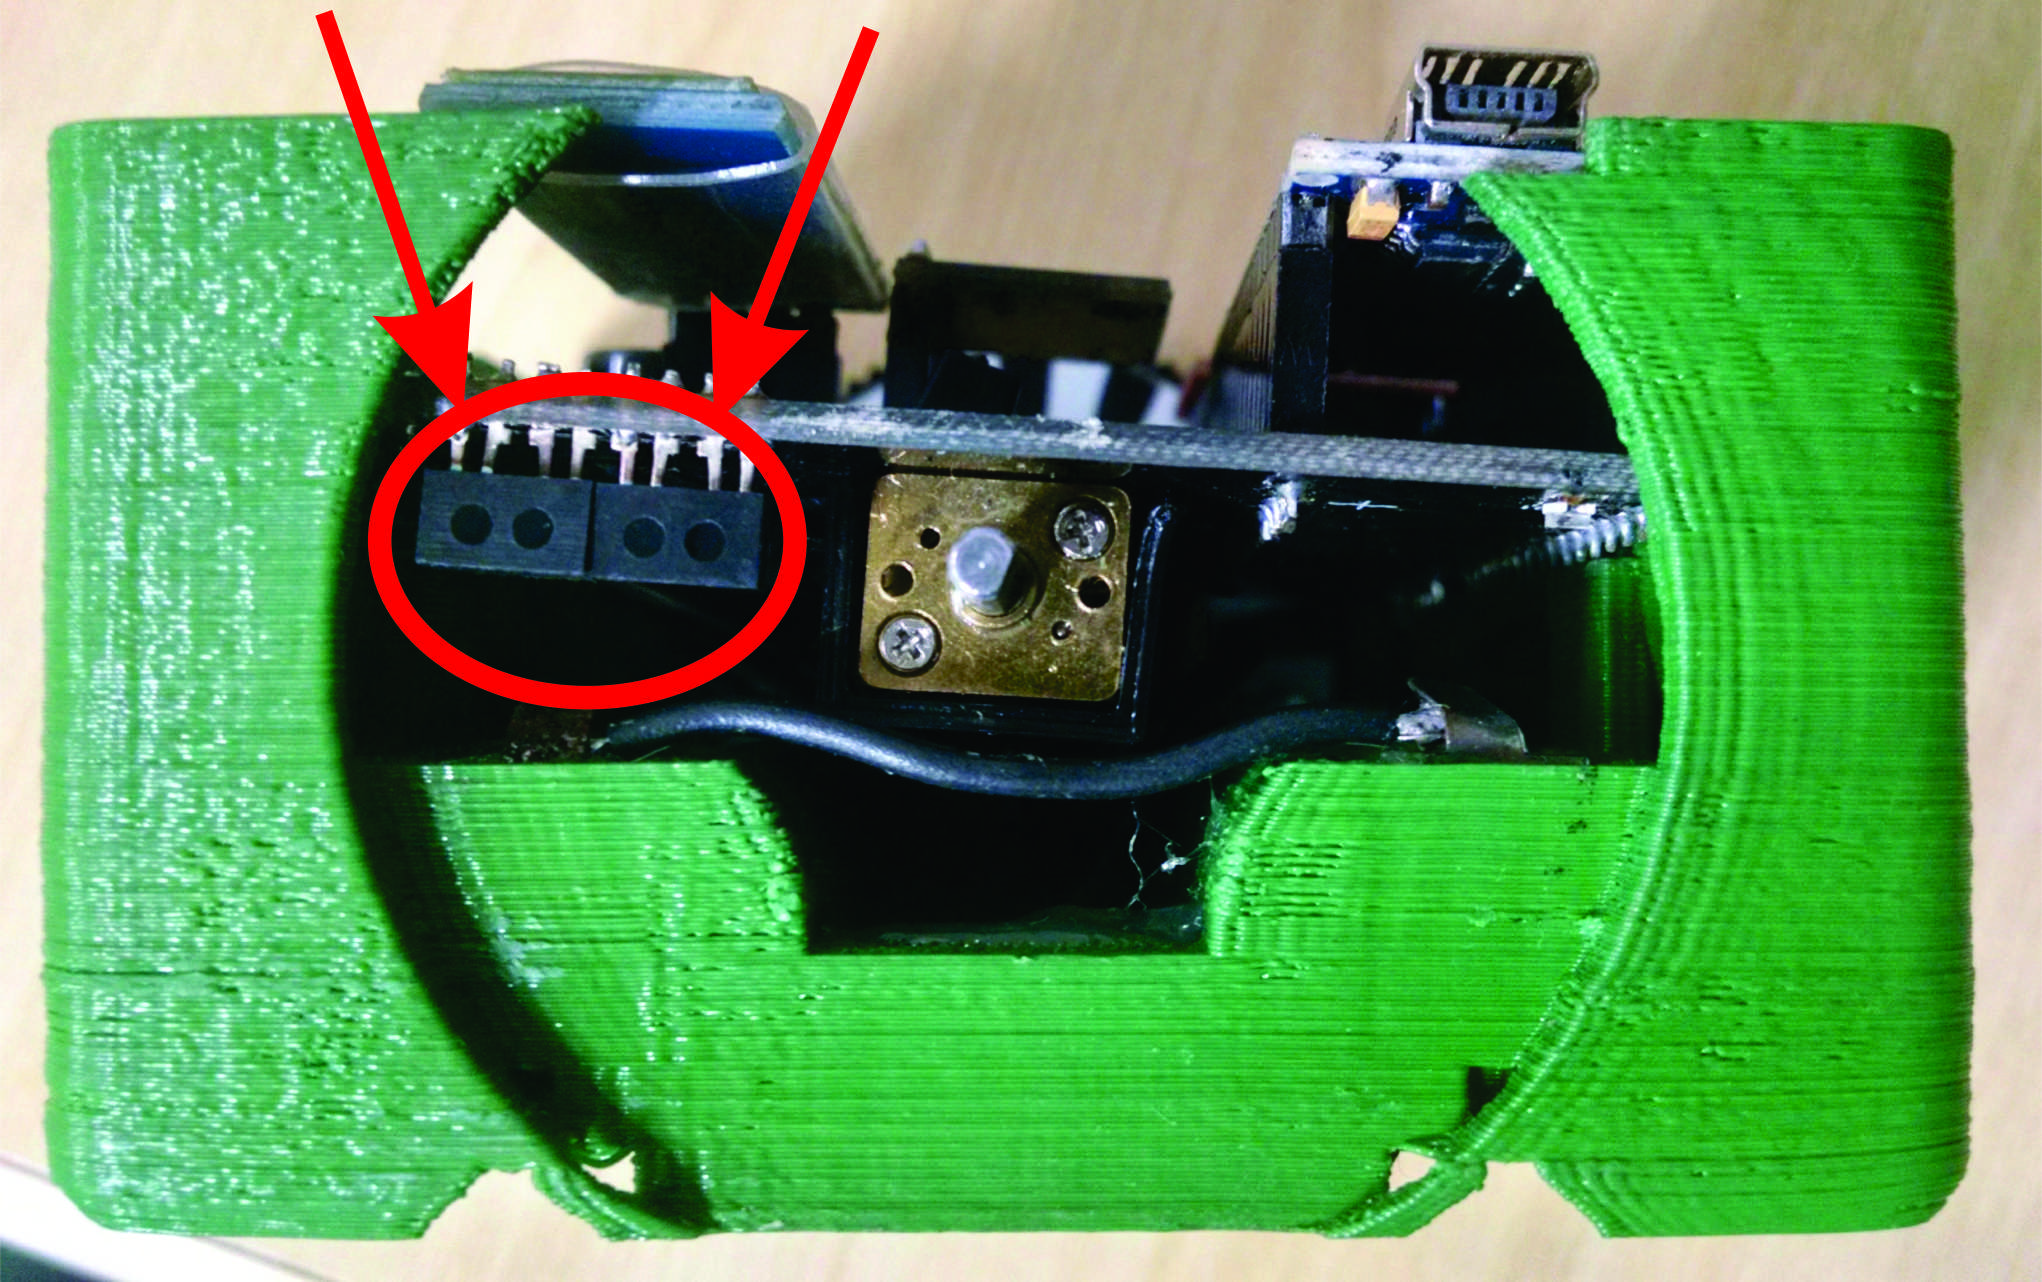
\includegraphics[width=0.5\textwidth]{lateralmodu.jpg}
	\caption{Vista lateral do robô Modu sem a roda, carcaça verde feita em impressora 3D. Em destaque: dois sensores ópticos ao lado do eixo de motor.}
	\label{fig:lateralmodu}
\end{figure}

\section{Roda}\label{roda}
O robô Modu possui um par de rodas, e em cada roda um adesivo com marcadores radiais preto e branco, como pode ser visto na Figura~\ref{fig:rodasmarc}.
\begin{figure}[H]
	\centering
	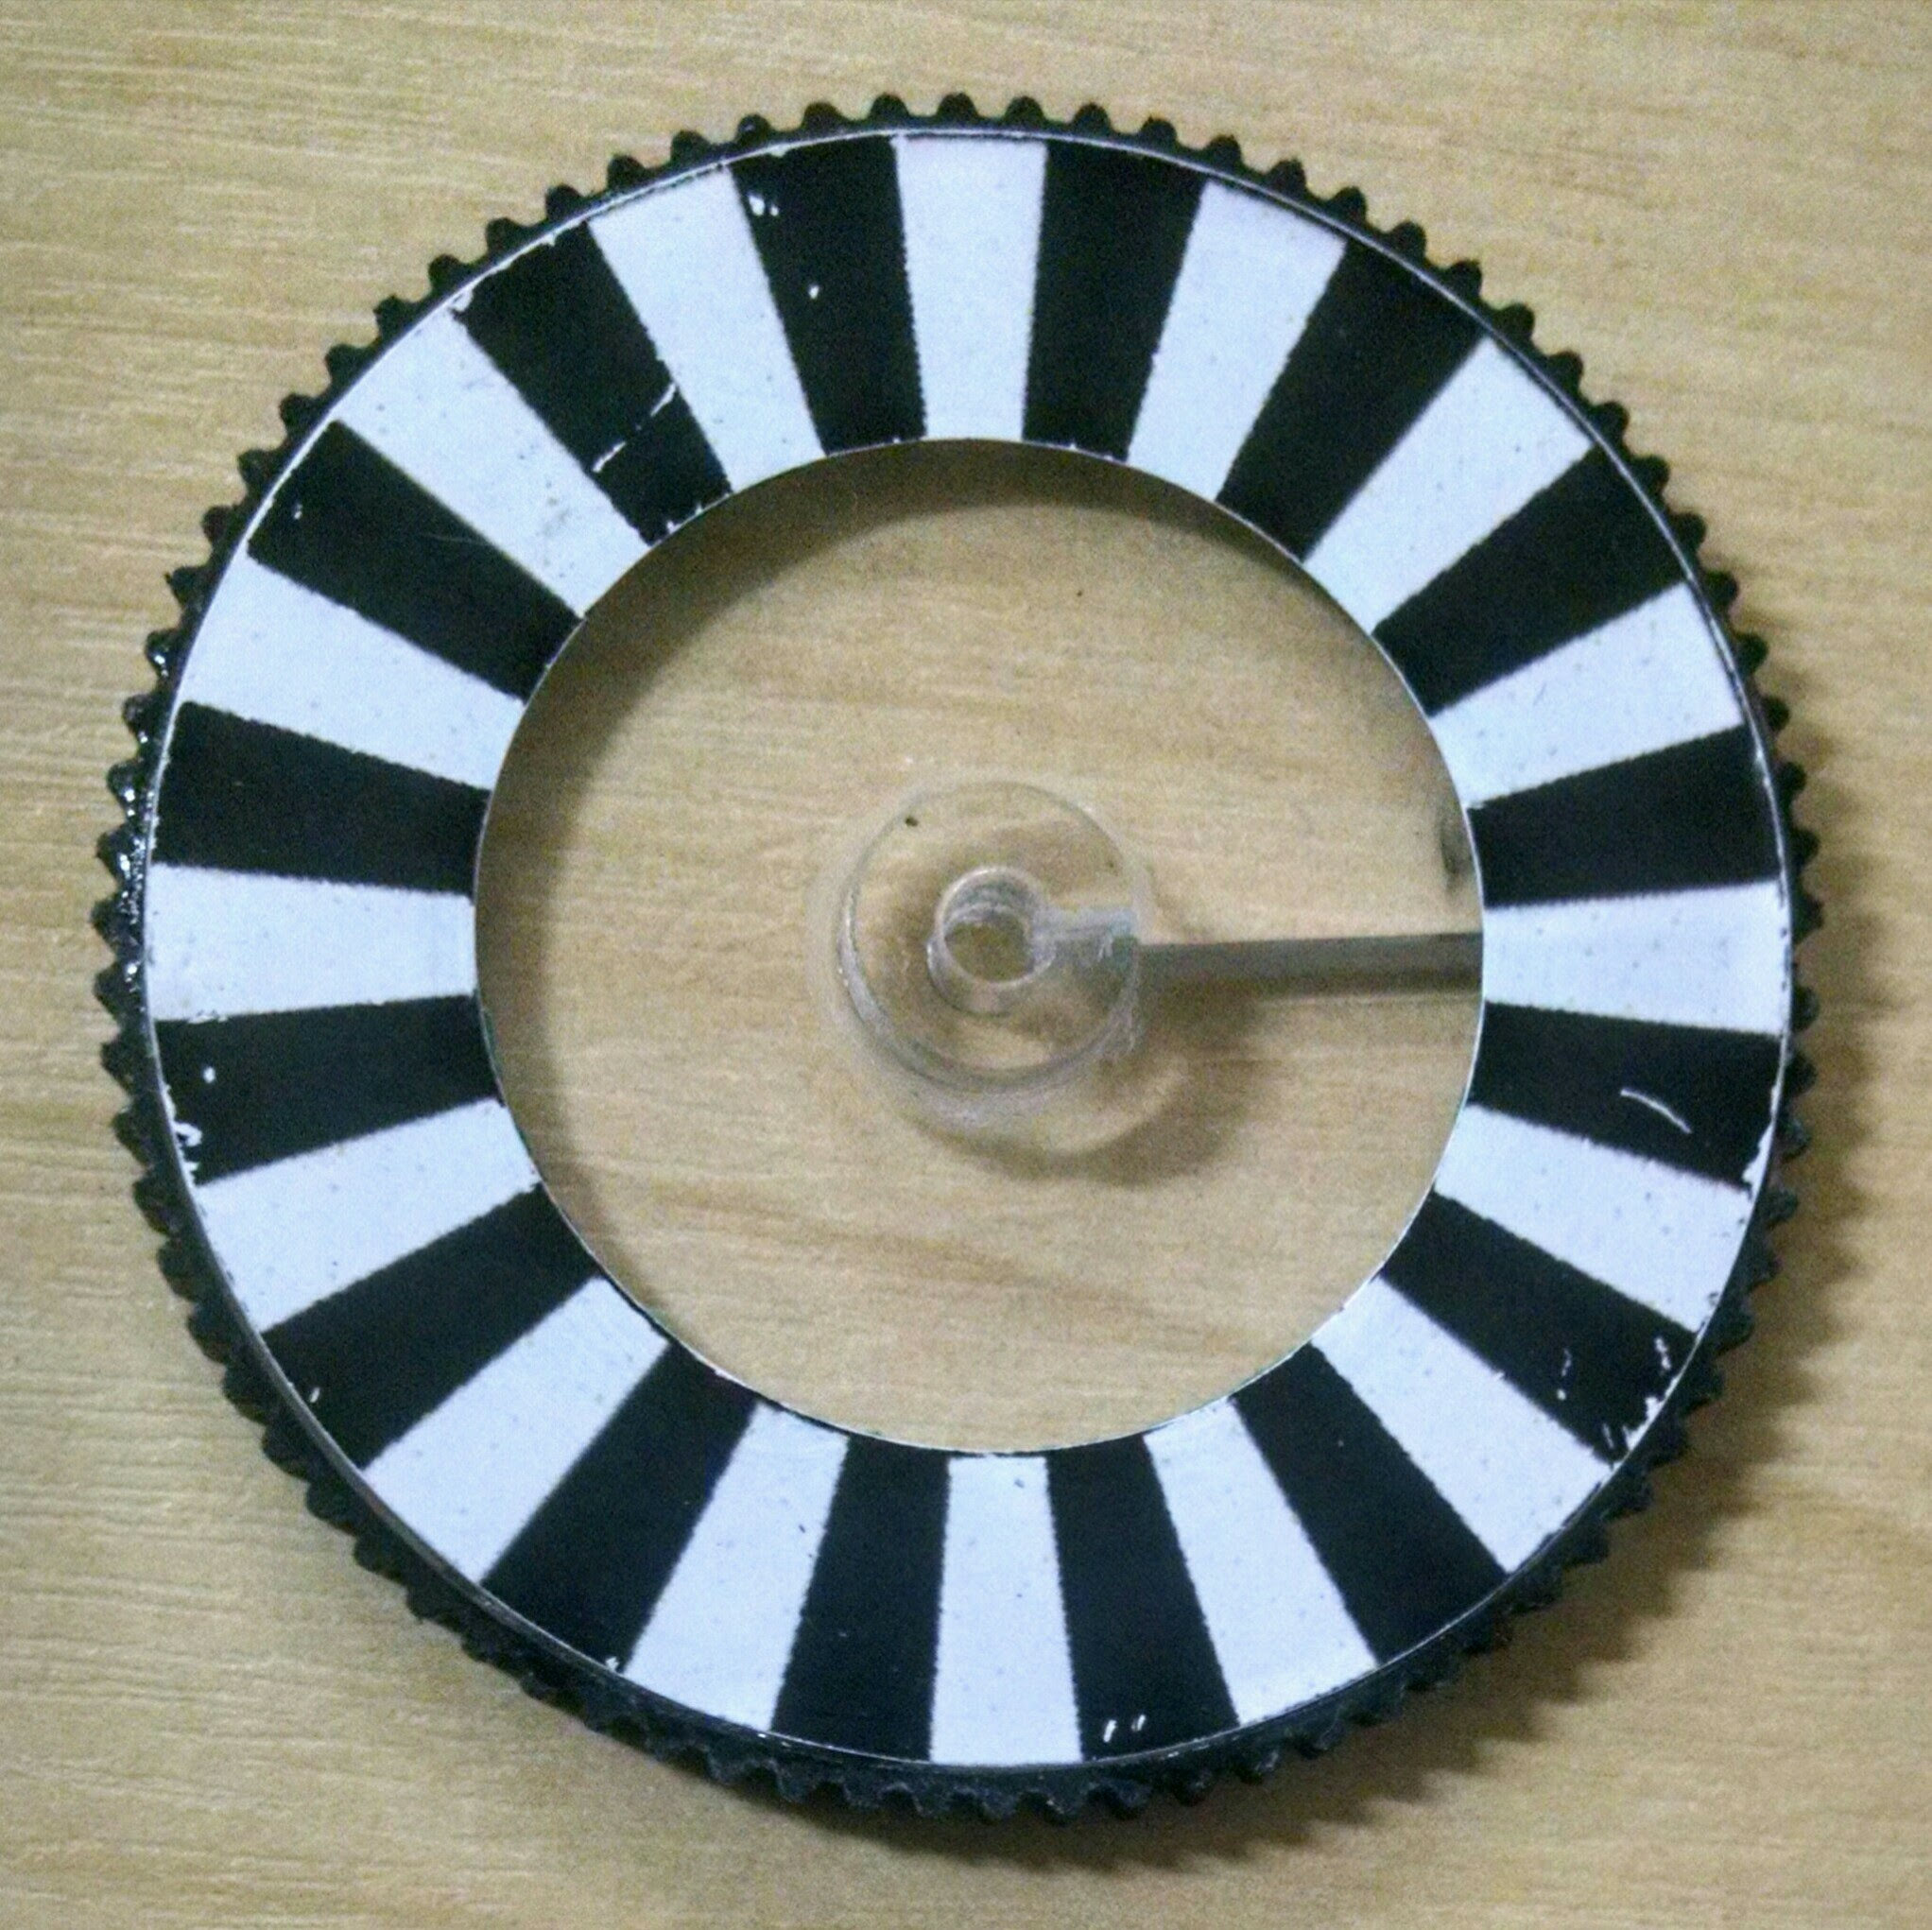
\includegraphics[height=0.32\textwidth]{roda32marc.jpg}
	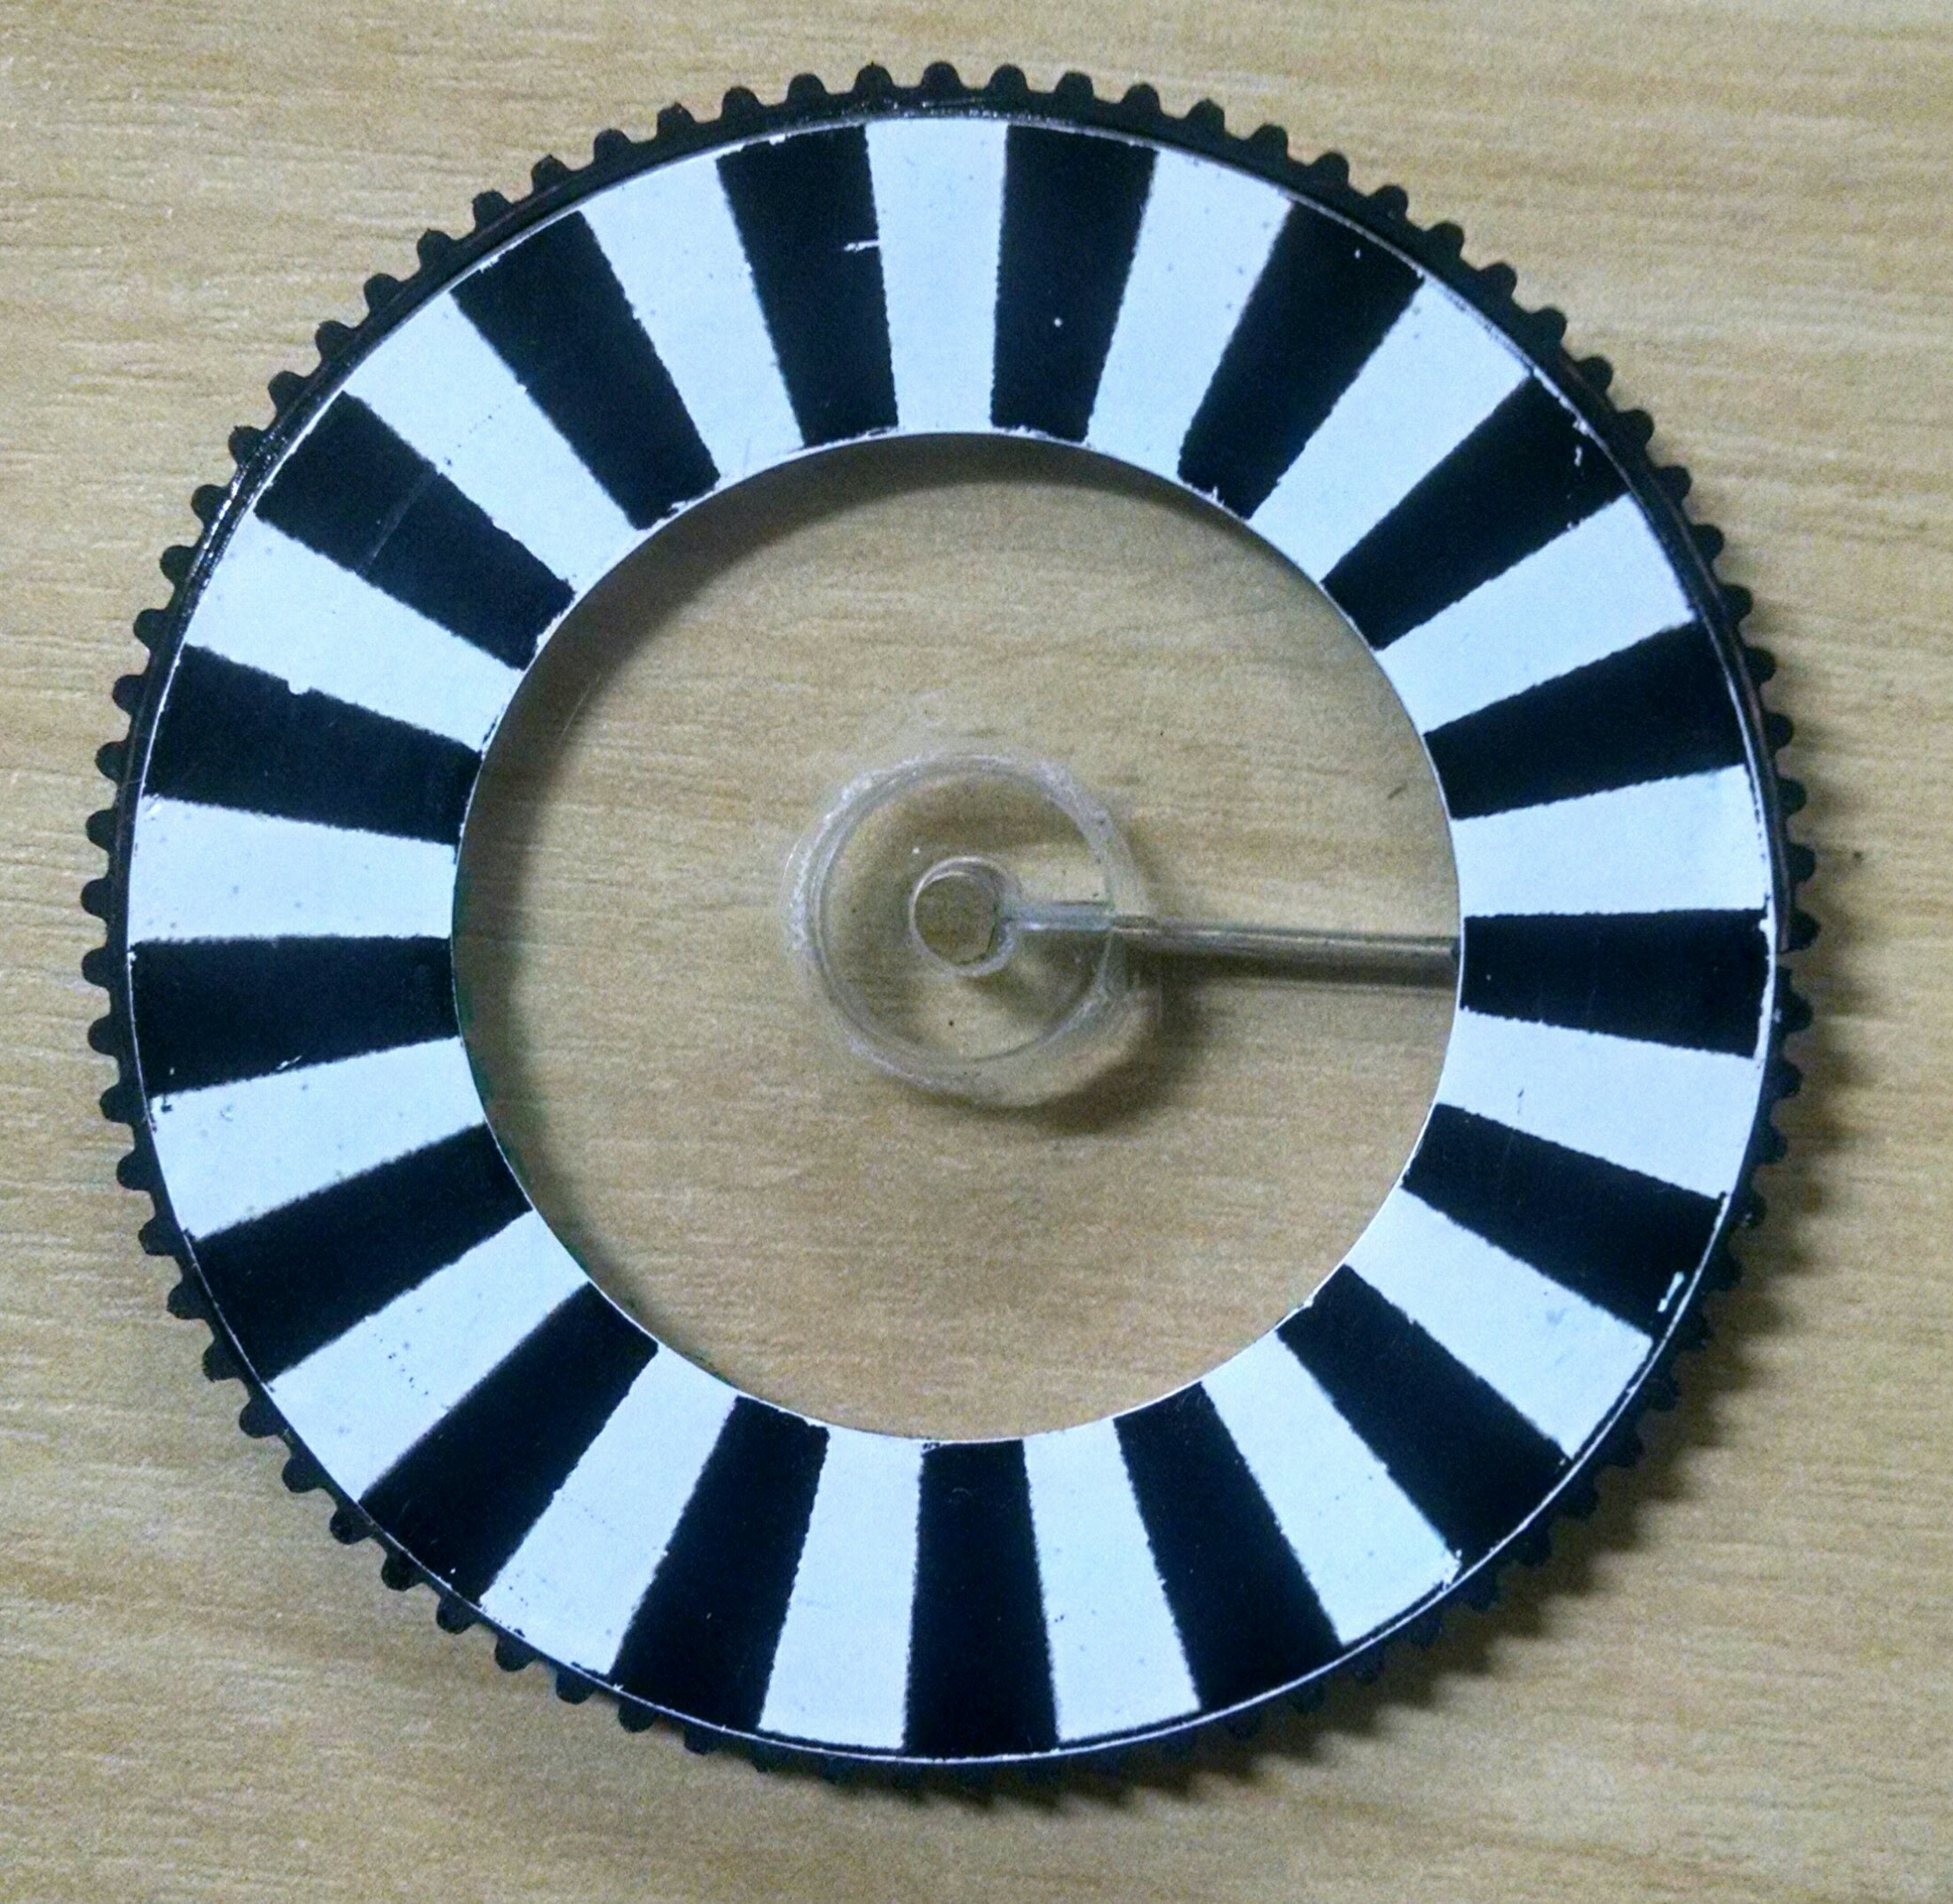
\includegraphics[height=0.32\textwidth]{roda34marc.jpg}
	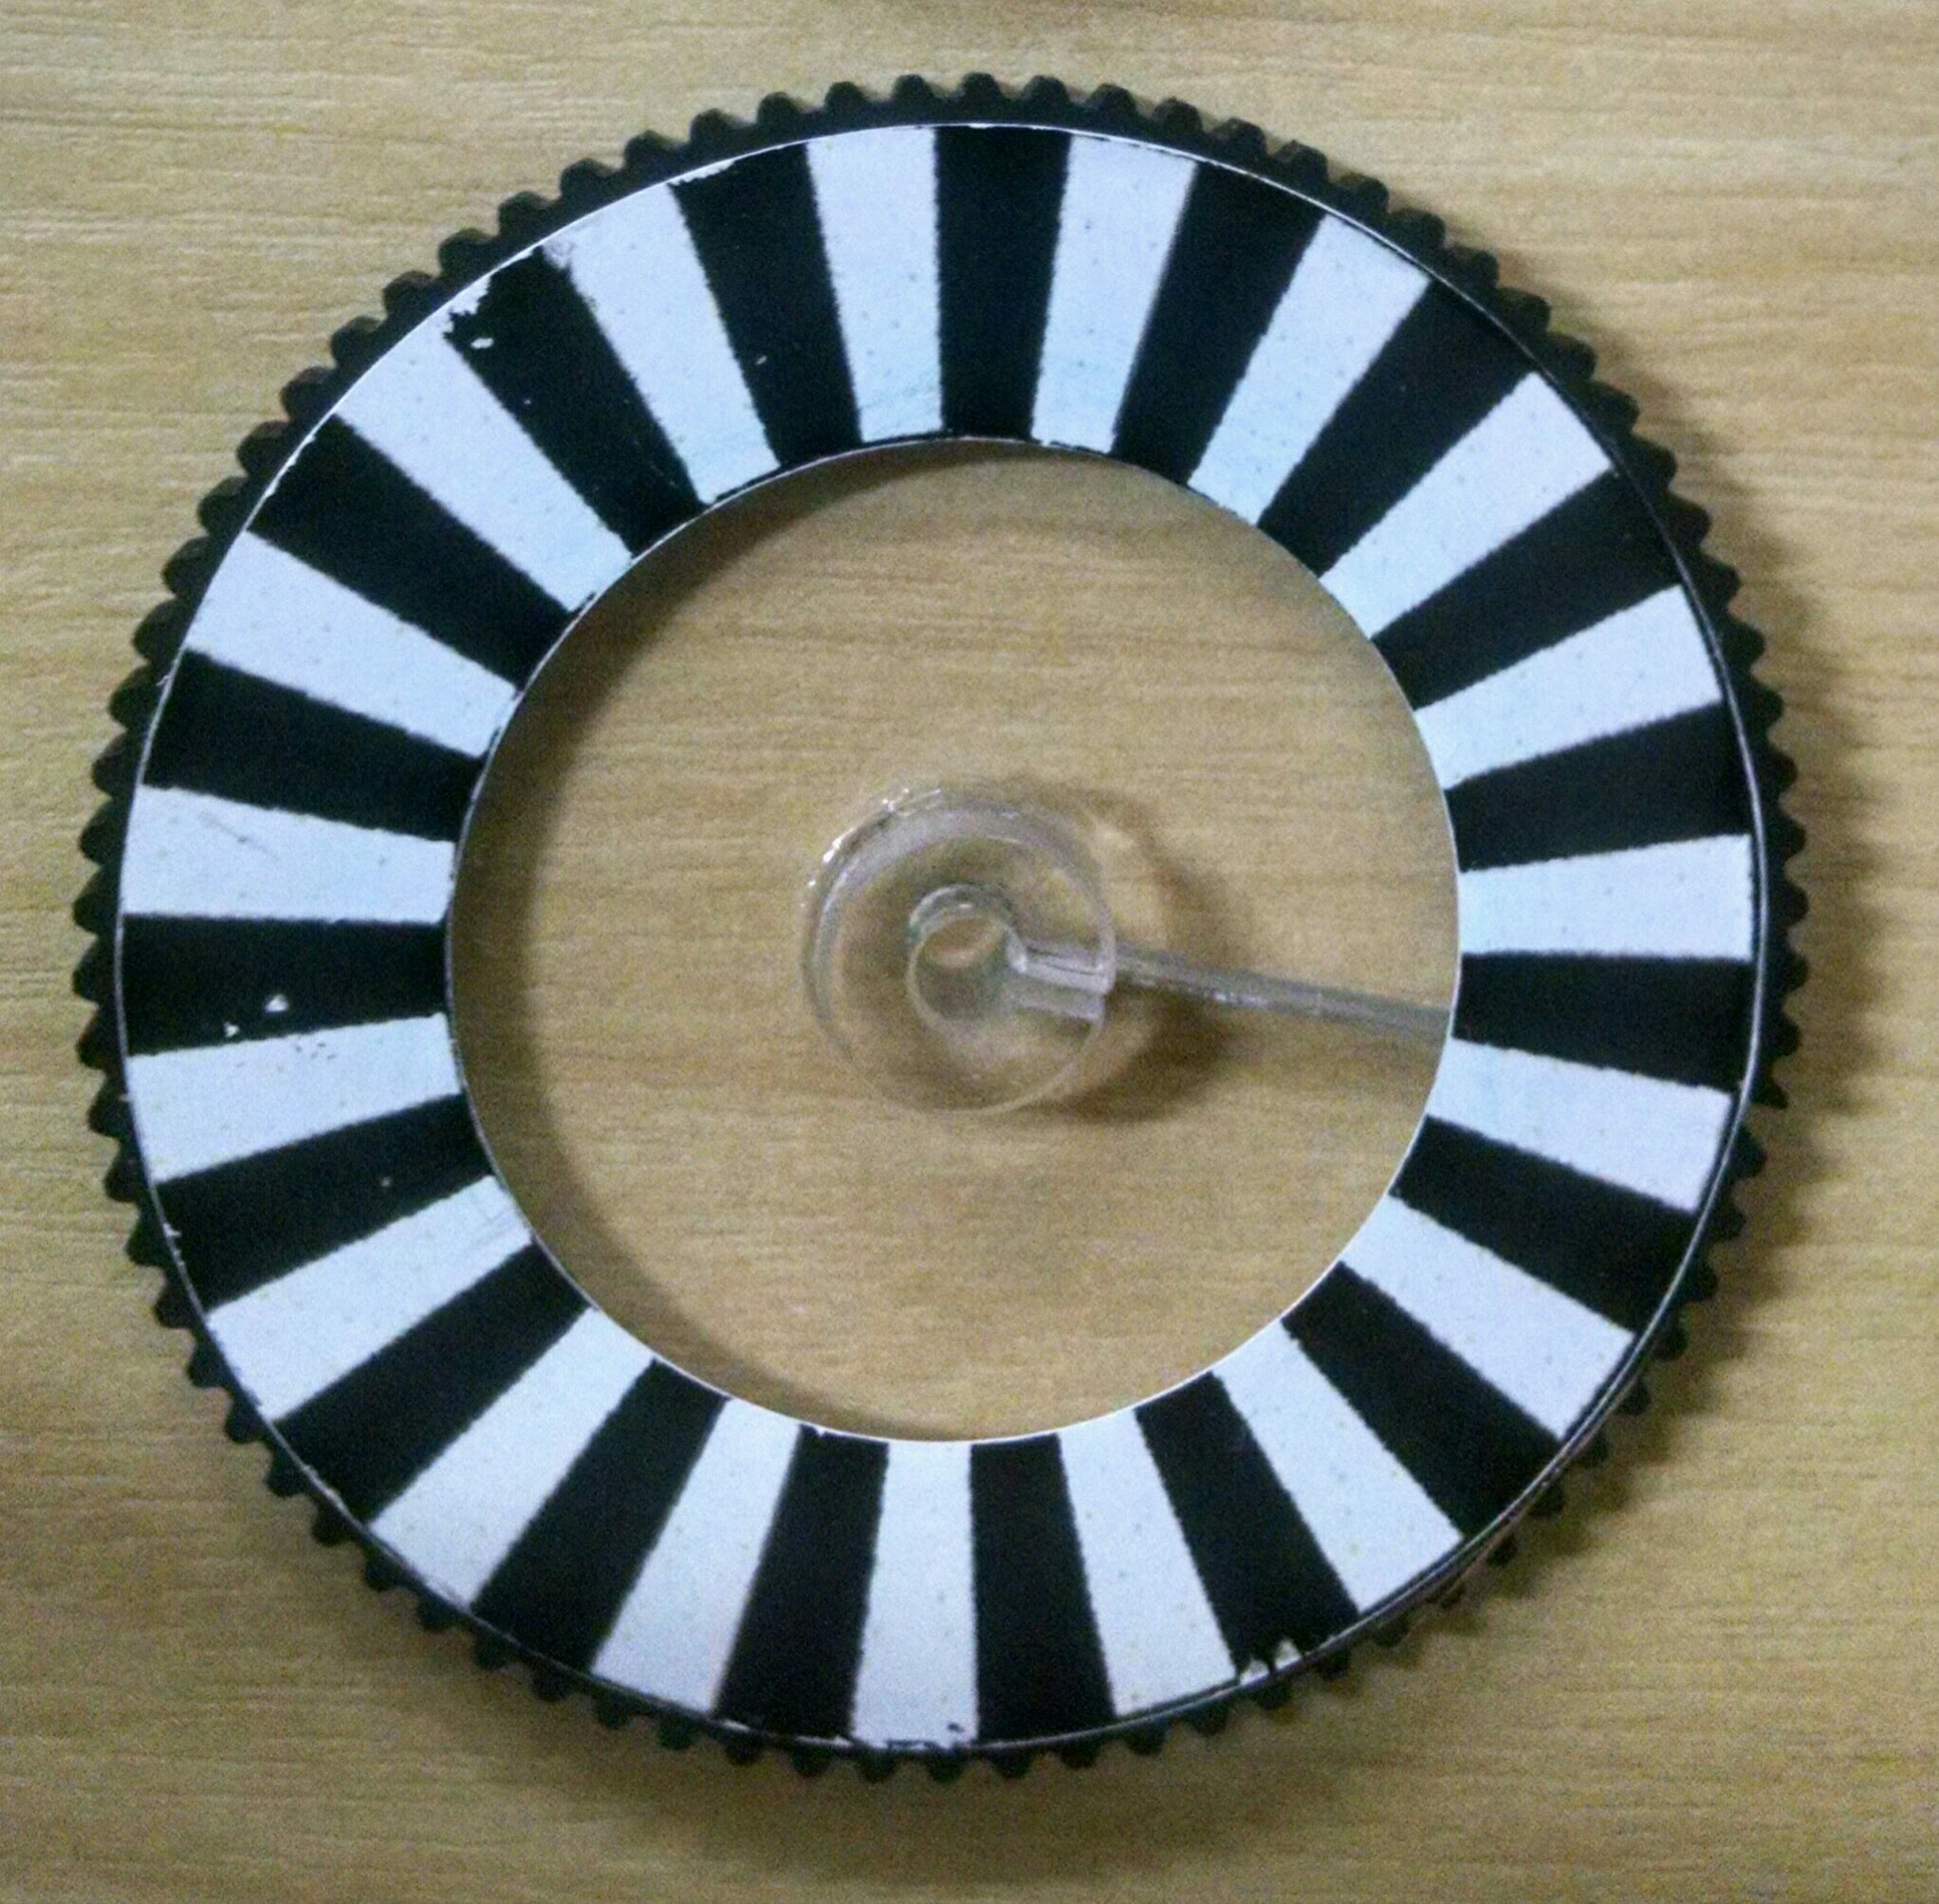
\includegraphics[height=0.32\textwidth]{roda38marc.jpg}\\
	(a)\hspace{0.32\textwidth}(b)\hspace{0.32\textwidth}(c)
	\caption{Roda com fita de 32, 34 e 38 marcadores, da esquerda para direita respectivamente.}
	\label{fig:rodasmarc}
\end{figure}
O conjunto composto pela roda, marcadores e sensores ópticos compõem o que denominamos de {\em encoder}. A precisão do \textit{encoder} pode ser ajustada aumentando ou diminuindo o número de marcadores.

\section{Encoder}\label{encoder}
Em resumo, \citeonline{braga2009funcionam} descreve um \textit{encoder} como um componente formado por transistores capaz de converter movimento linear ou angular em sinais digitais, dos quais geralmente são utilizados para determinar a posição, velocidade e em alguns, casos dependendo da configuração do \textit{encoder}, pode-se também determinar a direção de rotação do sistema. 

\section{Bluetooth HC-06}\label{bthc06}
O módulo Bluethooth (Figura~\ref{fig:BTHC06}) é utilizado para comunicação sem fio entre o robô e o computador ``técnico", a troca de informação ocorre utilizando-se comunicação serial. O alcance do módulo segue o padrão da comunicação bluethooth, aproximadamente 10 metros, o suficiente, visto que o campo de futebol de robôs da categoria VSS possui apenas dois metros e poucos centímetros Uma característica deste modelo (HC-06) é possuir apenas o modo de operação \textit{slave}, neste modo é apenas permitido receber conexão de outros dispositivos, ou seja, não permite que este modelo busque/solicite conexão com outros dispositivos, assim como ocorre com fones de ouvido e caixas de som.
\begin{figure}[H]	
	\centering
	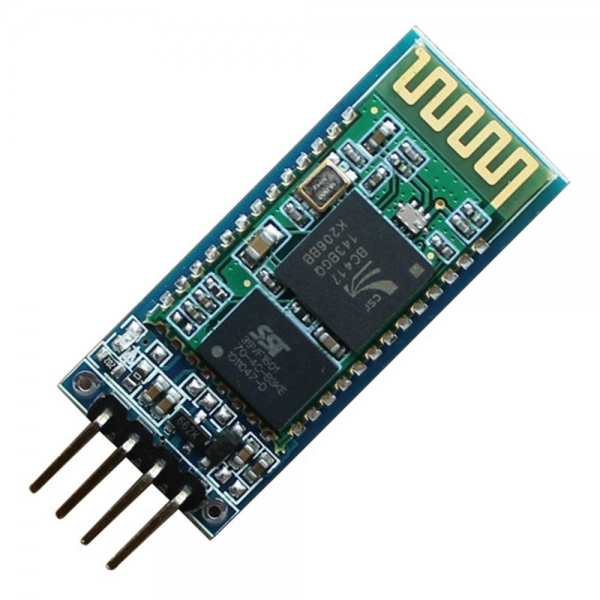
\includegraphics[width=0.5\textwidth]{BTHC06.jpg}
	\caption{Componente bluetooth modelo HC-06. Fonte:~http://buildbot.com.br}
	\label{fig:BTHC06}
\end{figure}

\chapter{Ambiente de desenvolvimento}
Este capítulo aborda as ferramentas utilizadas para o desenvolvimento da programação dos robôs jogadores. O sistema operacional escolhido foi o Ubuntu Gnome 17.04 64-bit, por ser uma distribuição linux o Ubuntu já possui os drivers USB para comunicação a placas de teste, a utilizada no projeto foi a placa Arduino Nano 328, com o driver USB, como o FTDI. Será descrito também neste capítulo a instalação e configuração dos softwares: IDE Arduino, IDE Clion 2017.1 e PlatformIO.

\section{Arduino IDE}\label{arduinoide}
O Arduino 1.8.3 (IDE) é um software \textit{open-source} para desenvolvimento de programas para Arduino. A utilização deste software torna fácil escrever códigos e subir (\textit{upload}) para a placa. O Arduino IDE tem suporte para Windows, Mas OS e para Linux. Ambiente foi desenvolvido em Java baseado no Processing e outros softwares open-source, com a utilização da IDE qualquer placa Arduino pode ser utilizada com poucas configurações~\cite{sitearduinoide}.

\subsection{Intalação}
Na pagina oficial do Arduino\footnote{https://www.arduino.cc/en/Main/Software} foi realizado o download conforme o sistema operacional, neste projeto, o ambiente Linux x64, ao selecionar o download é possível fazer uma doação para os desenvolvedores da IDE, visto que é um projeto \textit{open-source} e software livre, não tendo fins lucrativos, o mesmo depende dessa colaboração da comunidade para permanecer ativo e continuar expandido. Então a versão atual, neste momento a versão 1.6.10~\ref{fig:arduino.tar} para linux.
\begin{figure}[H]	
	\centering
	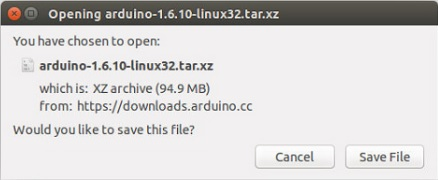
\includegraphics[width=0.5\textwidth]{dlArduino.jpg}
	\caption{Download IDE Arduino 1.6.10}
	\label{fig:arduino.tar}
\end{figure}
Ao finalizar o download do arquivo compactado, sera necessário descompactar~\ref{fig:arduinoextracao} em um diretório desejado, este ainda não sera o diretório de instalação. 
\begin{figure}[H]	
	\centering
	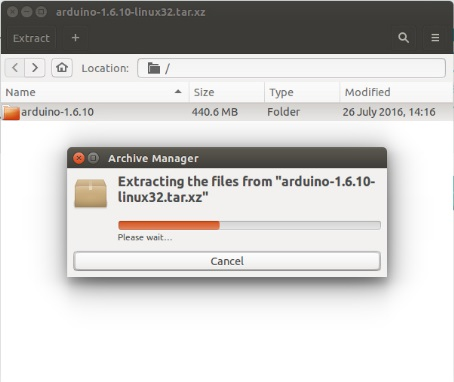
\includegraphics[width=0.5\textwidth]{unrarArduino.jpg}
	\caption{Extração dos arquivos do arquivo baixado}
	\label{fig:arduinoextracao}
\end{figure}
Abrindo o terminal deve-se navegar pelos diretórios utilizando o comando ‘CD’ até o diretório arduino-1.6.10 o qual foi criado ao descompactar o arquivo conforme a Figura~\ref{fig:caminhoidearduino}. Deve-se executar então o arquivo ``intall.sh" utilizando o comando: 
\begin{lstlisting}
./install.sh
\end{lstlisting}
O processo de instalação é rápido, e um novo ícone será criado na área de trabalho.
\begin{figure}[H]	
	\centering
	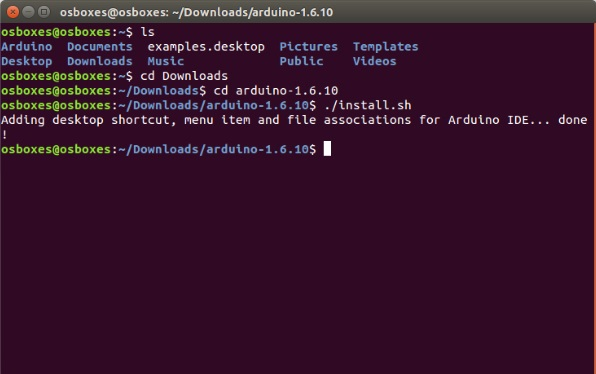
\includegraphics[width=0.5\textwidth]{installArduino.jpg}
	\caption{Comando CD para navegar entre as pastas e ./install.sh para instalação.}
	\label{fig:caminhoidearduino}
\end{figure}

\section{Clion 2017.1}
CLion é uma IDE multi-plataforma, criada pela empresa JetBrains para desenvolvimento de softwares nas linguagens C e C++. Suporte as linguagens nativas C e C++, incluindo C++11, C++14, libc++ e mais. A ferramenta desenvolvimento conta com ótimos recursos tais como: navegação, geração de código, gerenciamento de bibliotecas entre outros~\cite{siteclion}.

\subsection{Instalação}
Na página oficial de download do Clion\footnote{https://www.jetbrains.com/clion/download/\#\=linux} foi realizado o download do arquivo ``CLion-*.tar.gz" da versão compatível com o sistema operacional. Deve-se descompactar o arquivo ``CLion-*.tar.gz", no diretório /opt, e utilizado-se do seguinte comando para descompactar direto no diretório desejado.
\begin{lstlisting}
sudo tar xf CLion-*.tar.gz -C /opt/
\end{lstlisting}
Ao finalizar a descompactação, novamente deve-se acessar o diretório /bin, diretório este que se encontra junto aos arquivos descompactados, utilizando o comando: 
\begin{lstlisting}
cd /opt/CLion-*/bin
\end{lstlisting}
Executa-se então o arquivo clion.sh que se encontra dentro do subdiretório /bin, com o comando:
\begin{lstlisting}
./clion.sh
\end{lstlisting}

\section{PlatformIO}
Diferentes microcontroladores normalmente exigem diferentes ferramentas de desenvolvimento, para o Arduino temos a Arduino IDE. Outros usuários preferem ferramentas com auxílios, tais ambientes de desenvolvimentos como o Eclipse, o qual traz recursos que ajudam a gerenciar seus projetos, bibliotecas e funções de autocompletar. Com dificuldade em manter-se na linha com diferentes microcontroladores e ferramentas, o ecossistema (como é chamado pelos seus desenvolvedores) \textit{open-source} do PlatformIO agrupa tudo em uma única ferramenta. Sendo uma ferramenta multiplataforma podendo ser instalada nos sistemas operacionais Linux, Windows e MAC, fornece suporte a compilação para mais de 200 placas de teste, com mais de 15 plataformas de desenvolvimento e 10 \textit{frameworks}, incluindo as placas mais populares do mercado, organizando centenas de projeto e bibliotecas que podem ser incluídas no projeto~\cite{platiformio}.

\subsection{Instalação}
A instalação ou atualização no MAC e Linux é feita pelo terminal, apenas utilizando-se do comando (sudo pode ser requerido): 
\begin{lstlisting}
python -c "$(curl -fsSL https://raw.githubusercontent.com/platformio/platformio/master/scripts/get-platformio.py)"
\end{lstlisting}

\section{Iniciando um novo projeto}
Para criar um novo projeto primeiramente deve-se abrir a IDE Clion, deve-se criar um novo projeto na linguagem C++ clicando em \textit{File}, \textit{New Poject} então em \textit{Create}. Ao finalizar a criação do novo projeto, no menu de opções de configurações utilizando o atalho de teclado ``Ctrl + Alt + S" na aba ``\textit{Plugins}” (Figura~\ref{fig:tela1plugin}) no campo de texto procure por Arduino. Caso não seja localizado no repositório local utiliza-se do mecanismo de busca (\textit{Search in repositories}) para procurar nos repositórios da JetBrains, localizar os dois \textit{plugins} \textit{\textbf{Arduino}} e \textit{\textbf{Serial Port Monitor}} (Figura~\ref{fig:tela2plugin}).
\begin{figure}[H]	
	\centering
	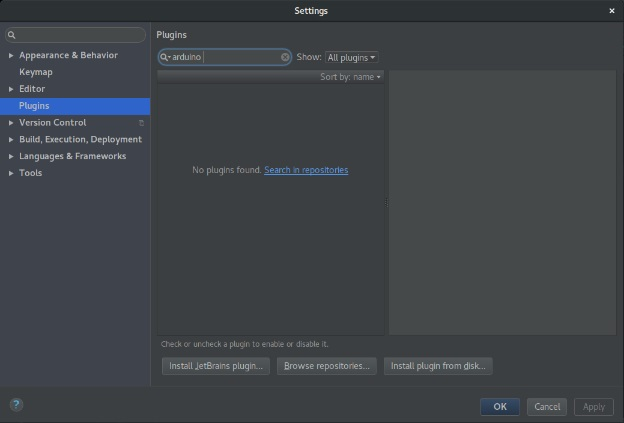
\includegraphics[width=0.5\textwidth]{pluginClion.jpg}
	\caption{Tela de busca de plugin.}
	\label{fig:tela1plugin}
\end{figure}
\begin{figure}[H]	
	\centering
	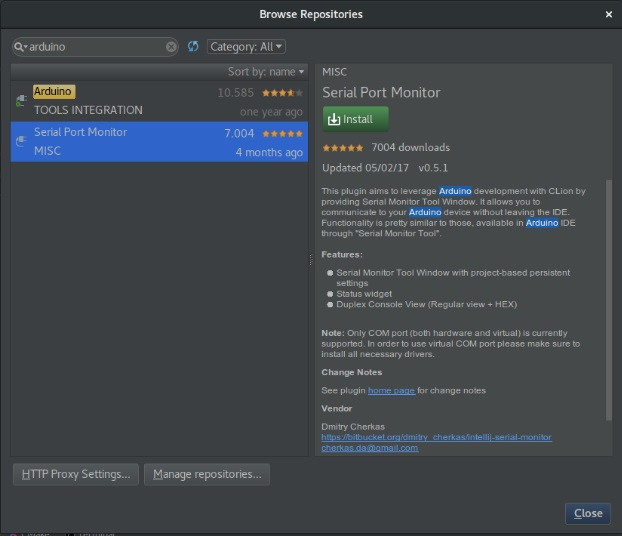
\includegraphics[width=0.5\textwidth]{pluginClion2.jpg}
	\caption{Tela com resultado da busca mostram os plugins a serem instalados.}
	\label{fig:tela2plugin}
\end{figure}
Após o termino da instalação dos dois plugins será necessário reiniciar o CLion para os \textit{plugins} possam funcionar. Com a IDE aberta, no terminal, deve-se navegar até o diretório do projeto criado. Neste projeto foi criado a pasta TCCTerceira no diretório de projetos do CLion o qual se encontra na home do linux.
\begin{lstlisting}
cd /home/kelvimro/CLionProjects/TCCTerceira
\end{lstlisting}
Ainda no terminal é utilizado o comando ``platformio” com a opção ``boards”, este comando lista as placas de teste suportadas pelo PlatformIO.
\begin{lstlisting}
platformio boards
\end{lstlisting}
Ao localizar a placa desejada na lista, Arduino Nano processador Atmel 328~\ref{fig:telananoatmega328}, utilizada no desenvolvimento dos robôs modelo MODU.
\begin{figure}[H]	
	\centering
	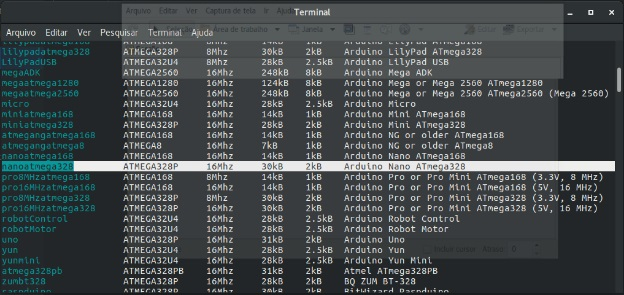
\includegraphics[width=0.5\textwidth]{boardPlatformio.jpg}
	\caption{Tela de seleção do modelo da placa ``nanoatmega328".}
	\label{fig:telananoatmega328}	
\end{figure}
Localizado e copiado o nome da placa ``nanoatmega328”, utilizando-se do comando ``\textbf{platformio}” com as opções de ``\textit{init}” para iniciar/instalar os recursos necessários no projeto,  a opção ``ide” deve-se utilizar o parâmetro ``\textit{clion}" indicando que será utilizado pelo framework o qual irá trabalhar em conjunto com a IDE do Clion, sendo assim o comando completo utilizado foi:
\begin{lstlisting}
platformio init --ide clion --board nanoatmega328
\end{lstlisting}
%\begin{figure}[H]	
%	\centering
%	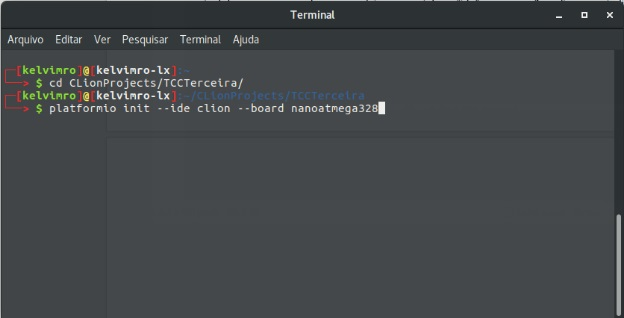
\includegraphics[width=0.5\textwidth]{initPlatformio.jpg}
%	\caption{Titulo.}
%\end{figure}
Finalizando a inicialização do PlatformIO será nescessário recarregar o arquivo CMake. Para isso deve-se clicar com o botão direito do mouse sobre o nome do projeto (TCCTerceira) e em seguida em ``\textit{Reload CMake Project}" (Figura~\ref{fig:reloadcmake}).
\begin{figure}[H]	
	\centering
	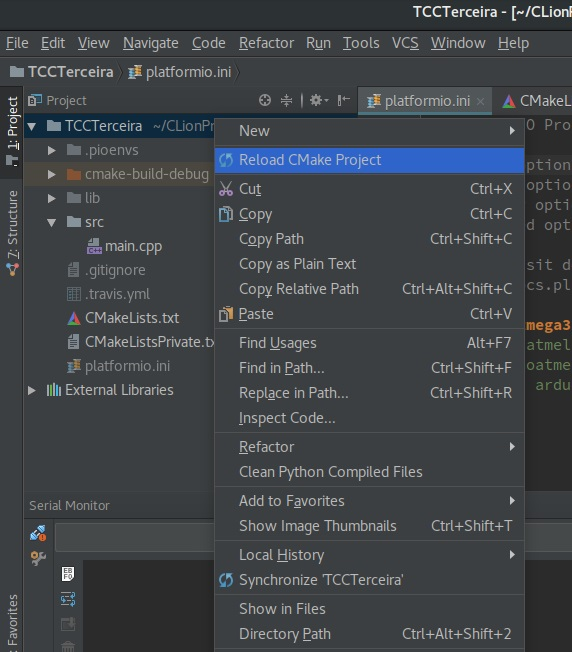
\includegraphics[width=0.5\textwidth]{reloadCmake.jpg}
	\caption{Opção de recarga do arquivo CMake do projeto.}
	\label{fig:reloadcmake}
\end{figure}
O PlatiformIO requer que as classes, assim como a Main.cpp, deve estar dentro da subpasta ``src" pois a ferramenta é configurada nativamente para buscar e compilar os códigos. Na classe Main.cpp deve-se importar a biblioteca ``Arduino.h" por meio do ``\#include".
\begin{lstlisting}
#include <Arduino.h>
\end{lstlisting}
O código a seguir foi utilizado para teste de compilação e funcionamento do ambiente como um todo ao finalizar a configuração. O programa tem a função básica, de piscar o led embutido na placa do arduino (LED\_BUILTIN) ou seja o pino da porta 13, ficando 1 segundo acesso e 1 segundo apagado.

\begin{lstlisting}
#include <Arduino.h>
void setup() {
// inicializa o pino digital LED_BUILTIN como saida.
pinMode(LED_BUILTIN, OUTPUT);
}

// Função loop do arduino
void loop() {
digitalWrite(LED_BUILTIN, HIGH);   // liga o LED 
delay(1000);                       // espera um segundo
digitalWrite(LED_BUILTIN, LOW);    // desliga o LED
delay(1000);                       // espera um segundo
}
\end{lstlisting}

Compilando o código utilizando Ctrl + F9 ou clicando no ícone no canto superior direito (Figura~\ref{fig:telarun1}).
\begin{figure}[H]	
	\centering
	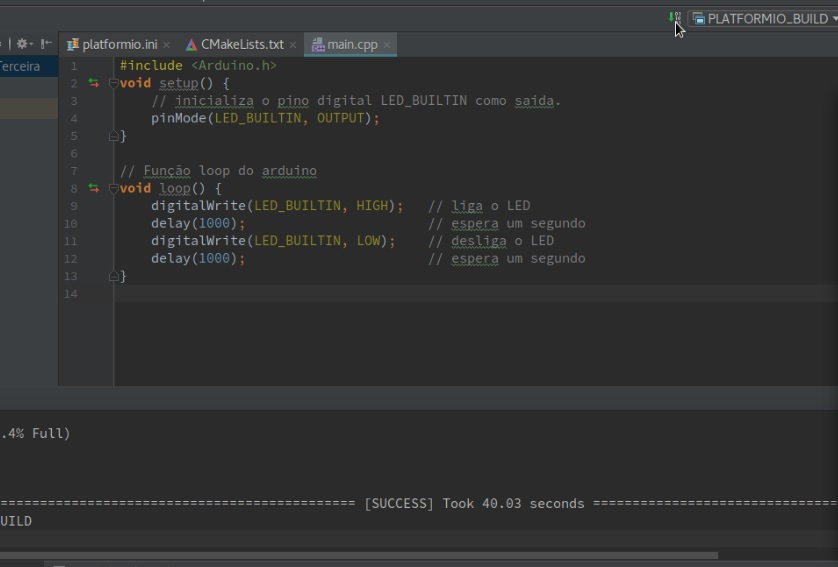
\includegraphics[width=0.5\textwidth]{buildClion.jpg}
	\caption{Tela principal, botão de compilação.}
	\label{fig:telarun1}
\end{figure}
Ao receber a mensagem de ``SUCCESS" (Figura~\ref{fig:telarun1})  na aba ``\textit{Messages}" , indica que o ``\textit{build}", ou seja, a compilação do programa foi concluída com êxito.
No fim a compilação (\textit{build}) é hora de carregar (\textit{upload}) do código para a placa arduino mudando para opção PLATFORMIO\_UPLOAD (na caixa de seleção no canto superior direito) utilizando-se do ícone ``\textit{PLAY}" verde~\ref{fig:telaupload}.
\begin{figure}[H]	
	\centering
	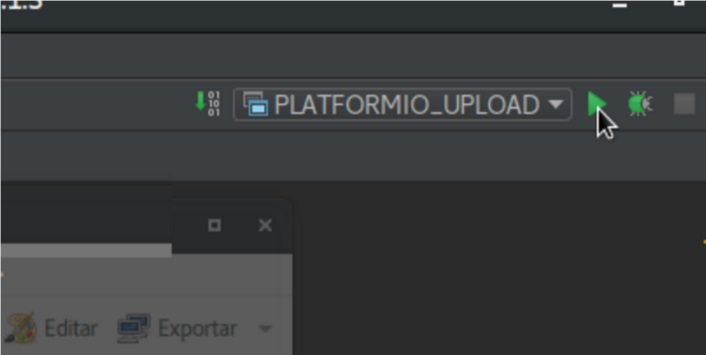
\includegraphics[width=0.5\textwidth]{upload.jpg}
	\caption{Botão utilizado para carregar (\textit{upload}) o programa no Arduino Nano.}
	\label{fig:telaupload}
\end{figure}
Na próxima mensagem de sucesso, a qual indicando que o programa já foi completamente enviado a placa, então o código já encontra-se em execução.
ATENÇÃO: Algumas distribuições podem solicitar a permissão de administrador para ter acesso ao dispositivo USB antes de fazer o upload do código. O privilégio pode ser concedido com a utilização do comando:
\begin{lstlisting}
sudo chmod 777 /dev/ttyUSB0
\end{lstlisting}
O numero “0” em \textbf{ttyUSB0} deve ser trocado conforme a porta ao qual o dispositivo foi conectado.

Em algumas distribuições as permissões devem ser fornecidas quando o dispositivo for conectado/reconectando.
Finalizando assim as configurações do ambiente de desenvolvimento, que foi utilizado para gerenciar e editar os códigos neste trabalho de conclusão.

\chapter{Interrupções no Atmega328}
%O processador Atmega328 que compõem o Arduino Nano, apresentado nesta seção discorreremos sobre o funcionamento da interrupção neste processador, utilização no projeto, exemplos e !!efeitos colaterais!!.

A maioria dos processadores possuem interrupções as quais permitem executar uma função após determinado evento externo, sendo chamado de interrupções externas. Nas referências presentes no site oficial do Arduino, de um modo didático e simples, faz-se um paralelo ao cotidiano, ao fazer o jantar e ter de cozinhar as batatas, é colocado um despertador com o tempo de 20 minutos, podendo fazer uma atividade paralela, durante o tempo de cozimento, ao despertar o alarme interrompe-se a atividade e então termina o jantar. 

Apesar do exemplo utilizado ser uma mudança de estado, não é recomendado invocar funções de interrupção que sejam grandes e complexas, pois além de sair da linha principal de execução, tais funções não contém argumentos, utiliza-se então variáveis do tipo voláteis. Logo, recomenda-se as interrupções para trocas de \textit{flag}, disparo de funções emergênciais, contagens precisas entre outros, pois a interrupção é como um ``botão vermelho''.

\section{Rotinas de serviço de interrupção (ISR)}\label{isr}
As rotinas de serviço de interrupção conhecidas pela sigla ISR, que vem do inglês \textit{Interruption Service Rotines}, encontram-se fora da função \textbf{loop}, ou seja, são funções as quais serão executadas quando ocorrer uma interrupção, interrompendo a execução do código \textbf{loop} e retornando ao ponto onde parou ao final da execução da ISR. \citeonline{simonmonk} destaca que:
\begin{quote}``Quando uma ISR está sendo executada, as interrupções são automaticamente desligadas. Isso evita com que as ISRs interrompam umas as outras."\end{quote}

Sendo assim, enquanto uma ISR estiver ativa outras não serão executadas.

\section{Modos de Interrupção}\label{modointerrupcao}
Os chamados modos de interrupção são como gatilhos que disparam ISR, ou seja, uma ISR é uma função a ser executada sempre quando o gatilho é acionado. O Atmega328 possui quatro modos de interrupção, são eles: \\
\begin{description}
	\item[\textit{LOW:}] Disparar uma interrupção continuamente enquanto o pino selecionado estiver em nível baixo (\textit{low}).
	\item[\textit{RISING:}] Dispara uma interrupção sempre que o pino passar de baixo (\textit{low}) para alto (\textit{high}).
	\item[\textit{FALLING:}] Dispara uma interrupção sempre que o pino passar de alto (\textit{high}) para baixo (\textit{low}).
	\item[\textit{CHANGE:}] Dispara uma interrupção sempre que o pino mudar de nível, em ambos os sentidos. 
	\item[\textit{HIGH}*:] Vale ressaltar que o modelo Arduino Due tem um quinto modo de interrupção, o \textit{HIGH}. Dispara uma interrupção continuamente enquanto o pino estiver em nível alto (\textit{high}).
\end{description}

\section{Prioridades das interrupções}\label{interrupcao328}
Assim como em outros processadores o Atmega328 possui sua lista de interrupções, é possivel observar a ordem de prioridade na Tabela~\ref{Tab:interrupcoes}, sendo que a de maior prioridade é interrupção \textit{reset}.

\begin{table}[!h]
	\renewcommand{\arraystretch}{1.3}
	\centering
	\begin{tabular}{|c|cc|}
		\hline
		1  &                      Reset                      &  \\ \hline
		2  &     External Interrupt Request 0  (pin D2)      &     (INT0\_vect)     \\ \hline
		3  &     External Interrupt Request 1  (pin D3)      &     (INT1\_vect)     \\ \hline
		4  & Pin Change Interrupt Request 0 (pins D8 to D13) &    (PCINT0\_vect)    \\ \hline
		5  & Pin Change Interrupt Request 1 (pins A0 to A5)  &    (PCINT1\_vect)    \\ \hline
		6  & Pin Change Interrupt Request 2 (pins D0 to D7)  &    (PCINT2\_vect)    \\ \hline
		7  &           Watchdog Time-out Interrupt           &     (WDT\_vect)      \\ \hline
		8  &         Timer/Counter2 Compare Match A          & (TIMER2\_COMPA\_vect) \\ \hline
		9  &         Timer/Counter2 Compare Match B          & (TIMER2\_COMPB\_vect) \\ \hline
		10 &             Timer/Counter2 Overflow             &  (TIMER2\_OVF\_vect)  \\ \hline
		11 &          Timer/Counter1 Capture Event           & (TIMER1\_CAPT\_vect)  \\ \hline
		12 &         Timer/Counter1 Compare Match A          & (TIMER1\_COMPA\_vect) \\ \hline
		13 &         Timer/Counter1 Compare Match B          & (TIMER1\_COMPB\_vect) \\ \hline
		14 &             Timer/Counter1 Overflow             &  (TIMER1\_OVF\_vect)  \\ \hline
		15 &         Timer/Counter0 Compare Match A          & (TIMER0\_COMPA\_vect) \\ \hline
		16 &         Timer/Counter0 Compare Match B          & (TIMER0\_COMPB\_vect) \\ \hline
		17 &             Timer/Counter0 Overflow             &  (TIMER0\_OVF\_vect)  \\ \hline
		18 &          SPI Serial Transfer Complete           &   (SPI\_STC\_vect)    \\ \hline
		19 &                USART Rx Complete                &   (USART\_RX\_vect)   \\ \hline
		20 &           USART, Data Register Empty            &  (USART\_UDRE\_vect)  \\ \hline
		21 &               USART, Tx Complete                &   (USART\_TX\_vect)   \\ \hline
		22 &             ADC Conversion Complete             &     (ADC\_vect)      \\ \hline
		23 &                  EEPROM Ready                   &   (EE\_READY\_vect)   \\ \hline
		24 &                Analog Comparator                & (ANALOG\_COMP\_vect)  \\ \hline
		25 &         2-wire Serial Interface  (I2C)          &     (TWI\_vect)      \\ \hline
		26 &           Store Program Memory Ready            &  (SPM\_READY\_vect)   \\ \hline
	\end{tabular}
	\caption[Lista de interrupções]{Lista de interrupções para o chip processador Atmega328. Fonte: gammon.com.au/interrupts}
	\label{Tab:interrupcoes}
\end{table}

As interrupções externas nomeadas como \textbf{INT0\_vect} e \textbf{INT1\_vect} que correspondem aos pinos digitais 2 e 3 respectivamente, no Arduino Nano (os pinos de interrupção podem mudar de acordo com a placa) sendo as maiores prioridades seguidas do \textit{reset}, é importante observar que observar as interrupções de 7 a 17 são interrupções de tempos e a interrupção de prioridade 25 é a interrupção para uso da interface serial.

\chapter{Desenvolvimento}\label{cap:desenvolvimento}
\section{Utilizando interrupção no Arduino}\label{usointerrupcao}
Nesta seção são apresentados os exemplos dos códigos utilizados no robô Modu para tratar as interrupções causados pelo \textit{encoder}. Conforme visto na Seção~\ref{interrupcao328}, os pinos de interrupção são o 2 e o 3, para isso foram utilizados duas variáveis:
\begin{lstlisting}
const int encodPinA1 = 2;                       // encoder A pino 2
const int encodPinB1 = 3;                       // encoder B pino 3
\end{lstlisting}
Dentro da função \textit{setup} configura-se os pinos como \textit{INPUT}, para que estes possam receber informações do sensor óptico:
\begin{lstlisting}
pinMode(encodPinA1, INPUT);
pinMode(encodPinB1, INPUT);
\end{lstlisting}
Segundo as referências disposta na documentação no site oficial do Arduino temos três sintaxes diferentes para acoplar\//iniciar, porém dentre elas apenas a seguinte é recomendada pelos desenvolvedores da IDE Arduino:
\begin{lstlisting}
attachInterrupt(digitalPinToInterrupt(pin), ISR, mode);
\end{lstlisting}
A função \textbf{digitalPinToInterrupt(pin)} é utilizada para traduzir o número do pino (\textbf{pin}) para o número específico da interrupção. O parâmetro \textbf{ISR} é o nome da função a ser chamada quando a interrupção ocorrer, a função não deve conter argumentos. O \textbf{mode} define o modo de ativação da interrupção, conforme descrito na Seção~\ref{modointerrupcao}.
Seguindo a sintaxe recomendada inicializa-se a interrupção com o pino e função desejada:
\begin{lstlisting}
attachInterrupt(digitalPinToInterrupt(encodPinA1), rencoderA, CHANGE);
attachInterrupt(digitalPinToInterrupt(encodPinB1), rencoderB, CHANGE);
\end{lstlisting}

Conforme o código acima, a função de nome \textbf{rencoderA} (\textbf{ISR}) será executada sempre que seu valor do pino \textbf{encodPinA1} (\textbf{pin}) mudar, pois seu modo foi definido como \textit{CHANGE} (\textbf{mode}), o mesmo acontece com o pino \textbf{encodPinB1} chamando sua respectiva ISR nomeada como \textbf{rencoderB}.

\begin{lstlisting}
	void rencoderA() {
	countA++;
	}
	void rencoderB() {
	countB++;
	}
\end{lstlisting}

Do mesmo modo que se pode acoplar uma interrupção a um pino específico, também é possível desacopla-lo utilizando o código a seguir sempre que achar necessário.

\begin{lstlisting}
detachInterrupt(digitalPinToInterrupt(encodPinA1));
detachInterrupt(digitalPinToInterrupt(encodPinB1));
\end{lstlisting}

O código acima é utilizado para desacoplar a interrupção do pino especifico \textbf{encodPinA1} e do pino \textbf{encodPinB1} respectivamente.

Existe um modo alternativo de ativar\//desativar as interrupções, mas estas funções ativam\//desativam todas a interrupções.

\begin{lstlisting}
interrupts();		// Ativa todas interrupções
noInterrupts();		// Desativa todas interrupções
\end{lstlisting}

Lembrando que, ao desativar as interrupções utilizando-se da função acima, as interrupções citadas na Tabela~\ref{Tab:interrupcoes} são todas desativadas, impedindo a utilização de quaisquer recursos que utilizem interrupções. Contudo, pode ser muito útil nos trechos de códigos sensíveis ao tempo. No código a seguir desativa-se as interrupções a fim de evitar que os valores da variável contadora sejam alterados durante a execução, evitando assim erros de leitura quanto as velocidades das rodas.
\begin{lstlisting}
	noInterrupts();				// Desativa interrupts
	calibA.push(countA);		// Adiciona a ultima contagem a fila de amostras
	countA = 0;					// Zera contadores de marcos do encoder
	calibMillis = millis();		// Zera o contador de tempo
	interrupts();				// Ativa interrupsts
\end{lstlisting}

Para mais informações a cerca de interrupções é indicado as notas de \citeonline{gammon} (https://gammon.com.au/interrupts).

\section{Controlador PID}\label{pid}
Nesta seção, está descrito o funcionamento do controle PID, abreviatura para Proporcional, Integral e Derivativo, e como utilizá-lo em aplicações de controle que requer controle de precisão~\cite{controlepid}. Como exemplo, considere  um carro que tenta manter uma distância X do carro da frente.

\subsection*{P - Proporcional}
Ao tentar manter uma distância X o carro de trás deve acelerar proporcionalmente quando o carro da frente acelerar e começar se distanciar, tentando alcançar o mesmo. No entanto, caso o carro de trás venha acelerar mais que o carro da frente a distância será menor que a desejada, X, então a nova correção é frear para aumentar a distância buscando ajustar a distância desejada de X. Novamente, caso a correção, que desta vez é a frenagem (desaceleração), for excessiva, a sua distância será superior a distância desejada de X, então novamente terá de acelerar. Isso ocorre indefinitivamente caso a aceleração não proporcional não esteja correta, ou seja, acelerando demais e freando de menos e não atingindo o ponto alvo (\textit{set point}). Então esta aceleração é chamada de ganho ou proporcional (P) em um controle PID.

\subsection*{I - Integral}
A integral, neste exemplo dos carros, seria como recuperar a distância X a cada instante, caso o veículo da frente venha a acelerar, o veículo de trás acelera gradualmente a fim de atingir a distância X com mais suavidade.

\subsection*{D - Derivativo}
A derivada é utilizada para eliminar erros acumulados na integral, neste exemplo dos carros, seria quando o carro de trás percebe que a distância desce ou decresce muito rapidamente em relação a desejada X, deixando as correções da integral ainda mais suaves, diminuindo a oscilação das correções em volta do \textit{set point}.

\subsection{Utilização do PID}
O controle do tipo PID é empregado para controlar a velocidade da roda mais rápida em relação a mais lenta, o controle PID se utiliza de dados obtidos durante em tempo de execução. Com um ciclo de atualização de 200 milissegundos (ms), ou seja, a cada 200 ms o controle obtém a velocidade de rotação de ambas as rodas, utiliza a velocidade do motor mais lento como \textit{set point} do motor mais rápido, calcula a proporcional, a integral e derivativo e utiliza o resultado como o novo valor do PWM do motor mais rápido o deixando com a velocidade de rotação mais próxima do motor de menor velocidade.

\subsection{Problemas no ciclo}
Durante o uso do controle PID para equalizar as velocidades dos motores foi percebido que o tempo de ciclo para o controle se tornar eficiente é superior ao intervalo de comandos recebidos pelo computador técnico o qual envia novos comandos com intervalo de 200 ms. O controle do tipo PID não consegue equalizar as velocidades na primeira correção, ao se aproximar da segunda ou terceira correção o robô recebe a próxima instrução mudando todas as referências de velocidades.

\subsection{Problemas devido interrupções}
O controle tipo PID requer o aferimento constante da velocidade por meio do \textit{encoder}, este gera interrupções, parando temporariamente (até que se finalize a ISR), trazendo discrepância nas contagens devido a perda de interrupções.
Conclui-se então que a utilização de controle do tipo PID do modo implementado não é recomendado, pois ao ser utilizado, os dois \textit{encoders} ao mesmo tempo e com grande velocidade nas rodas algumas interrupções são perdidas enquanto outra ISR já esta sendo executada.

\section{Ferramenta Monitoramento/Ajuste}
Nesta seção será apresentada o estudo e desenvolvimento da ferramenta para monitoramento e ajuste da velocidade das rodas do robô Modu. 

Um controle utilizando-se de pesos é de simples funcionamento, cada motor tem seu peso o qual é multiplicado pelo PWM correspondente recebido do computador técnico, com a diferença dos pesos, os motores com potência real diferente tendem a rodarem com velocidades muito próximas. 

%Para determinar valores dos pesos, inicia-se com coleta de amostras em seguida calcula-se a média das amostras adquiridas e por fim calculando os pesos para cada motor, surgindo então a ferramenta de calibragem por peso.
A ferramenta tem como principal finalidade determinar os valores dos pesos a partir de testes reais, utilizando a sintaxe da Seção~\ref{sintaxe} pode-se calcular os pesos, utilizando-se de um ou mais valores de PWM conforme a necessidade.
 
\subsection{Sintaxe da ferramenta}\label{sintaxe}
Neste trabalho foi criada uma ferramenta com sintaxe de comandos próprios, pode ser alterada nas primeiras linhas do código na qual encontramos as seguintes variáveis:
\begin{lstlisting}
#define START_CMD_CHAR '*'
#define DIV_CMD_CHAR '|'
#define CALIB_CMD_CHAR '@'
\end{lstlisting}

\subsection*{\textbf{START\_CMD\_CHAR}}\label{stardcmd}
\textbf{\textit{START\_CMD\_CHAR}} é o caractere que determina o início de uma mensagem de movimentação, seguido de dois inteiros (um inteiro para cada motor) separados pelo caractere \textbf{DIV\_CMD\_CHAR}, utilizando-se conforme a Tabela~\ref{Tab:exemplosintaxe}.

\begin{table}[!h]
	\renewcommand{\arraystretch}{1.3}
	\centering
	\begin{tabular}{|c|cc|c|}
		\hline
		 Comando   & Potência Motor A & Potência Motor B &    Movimento    \\ \hline
		 *100|100  &  100\% a frente  &  100\% a frente  &   Para frente   \\
		*-100|-100 & 100\% para trás  & 100\% para trás  &    Para trás    \\
		 *50|-50   &  50\% a frente   &  50\% para trás  & Rotação horária \\
		  *50|25   &  50\% a frente   &  25\% a frente   & Curva a direita \\ \hline
	\end{tabular}
	\caption[Comandos]{Tabela com exemplo de sintaxe para movimentação do robô}
	\label{Tab:exemplosintaxe}
\end{table}

\vspace{1.0cm}

O caractere inicial pode ser alterado para o caractere de identificação do robô, caso tenhamos mais que um robô controlado pelo mesmo rádio, obrigatoriamente o caractere inicial não pode ser um caractere do tipo inteiro (\textbf{\textit{INT}}), ou seja, tendo os robôs 'A','B' e 'C' com apenas um rádio pode-se comandar os três robôs no mesmo canal de comunicação se for alterado o \textbf{START\_CMD\_CHAR} de cada robô para seu respectivo ID, o sistema então ignora-rá os comandos pertencentes a outros robôs.

\subsection*{{DIV\_CMD\_CHAR}}\label{divcmd}
O caractere de divisão é utilizado como conector e serve exclusivamente para separar os números inteiros referentes aos valores de PWM. O \textbf{DIV\_CMD\_CHAR} deve ser único e pode ser alterado, mas nunca por um inteiro.

\subsection*{CALIB\_CMD\_CHAR}\label{calibcmd}
O caractere \textbf{CALIB\_CMD\_CHAR} é o caractere que identifica que os inteiros seguintes serão utilizados para calibragem e não para movimentação, sendo assim o caractere \textbf{CALIB\_CMD\_CHAR} invoca a função \textbf{calibrate()} (Seção~\ref{calibrate}). Este deve ser único e pode ser alterado, mas nunca por um inteiro.
Para solicitar uma calibragem o comando deve começar com, o caractere de calibragem, seguindo por 'N' inteiros separados por \textbf{DIV\_CMD\_CHAR} conforme os exemplos abaixo:
\begin{lstlisting}
	@100
	@100|150|200|255
	@150|150|150|150|150|150|150
\end{lstlisting}
Como pode ser visto no exemplo a cima, a função de calibragem aceita um número variável de PWMs, podendo calibrar em várias potências ou em uma mesma potência repetidas vezes, quanto maior o número de PWMs testados maior a precisão dos cálculos pois, dado que, quanto maior o número de amostras menor o erro.

\subsection{Calibragem - calibrate()}\label{calibrate}
A função de calibragem (\textbf{calibrate()}) é invocada com o uso do caractere \textbf{CALIB\-\_CMD\_CHAR} esta função recebe um ou mais valores de PWM e os testam.
\begin{lstlisting}
	// Coleta todos os PWMs do array
	while (Serial.available()) {
		pwmArray.push(Serial.parseInt());
	}
	while (!pwmArray.isEmpty()) {
		static int _pwm;
		_pwm = pwmArray.pop();
		getAmostras(_pwm);
	}
\end{lstlisting}

O primeiro laço de repetição \textit{while} é responsável por separar os valores de PWM e coloca-los em uma pilha, este trecho do código permite que a função teste números variados de PWMs.
No segundo \textit{while} é desempilhado um valor de PWM e este é utilizado na função \textbf{getAmostras(int \_PWM)} coletando o número de amostras para todos os PWM solicitados. Com as amostras coletadas é invocada a função \textbf{finalMedia()} \ref{finalMedia} para a conclusão da calibragem.

\subsection{Coleta de amostras - getAmostras(int \_PWM)}\label{getamostras}
Foi desenvolvido um método chamado \textbf{getAmostras(int \_PWM)} tendo como argumento o PWM desejado para coleta de amostras.
O método então coleta o número de amostras determinado na variável \textbf{NUM\_AMOSTRA} de escopo global como pode ser visto na linha 2 do código abaixo, pode-se verificar a variável \textbf{CALIBMILLIS} a qual determina intervalo de tempo para cada amostras. Afim de evitar erros na contagem devido a interrupções, as contagens são executadas separadamente, ou seja, primeiro é colhido as amostras do motor A e depois colhida as amostras do motor B.

\begin{lstlisting}
	// Numero de amostras para a media movel
	int NUM_AMOSTRA = 15;
	// Tempo de coleta de amostras
	const int CALIBMILLIS = 1000;
\end{lstlisting}

Usando-se a configuração acima, serão contados quantas interrupções foram geradas pelo \textit{encoder} em um intervalo de 1000 ms, gerando então uma amostra. 
Apresenta-se o código da função na íntegra, a variável \textit{print} é do tipo \textit{String} e tem escopo global para armazenar informações a serem utilizadas posteriormente. 
É importante salientar que o processo de comunicação Serial também gera interrupções e, portanto, deve ser evitado durante o processo de contagem.

Ao final da fase de coleta de amostras de ambos os motores, antes de retornar a função, um método chamado \textbf{processMedia()} é invocado para calcular a média das 15 amostras de cada motor. Uma descrição detalhada da função \textbf{getAmostras(int \_PWM)} pode ser vista no Apêndice~\ref{anexo:getamostra}.

\subsection{Média de amostas - processMedia()}\label{processmedia}
A função tem por finalidade computar a média para cada roda, será executada sempre que a função \textbf{getAmostras(int)} for invocada, utilizando-se das amostras já obtidas.
\[ vetMedias = \dfrac{\sum_{i=1}^{NUM\_AMOSTRA}amostra}{NUM\_AMOSTRA}   \]

\subsection{Determinação dos Pesos - finalMedia()}\label{finalMedia}
A função chamada \textbf{finalMedia()} é a último passo a ser executado na obtenção dos pesos. Esta tem como principal objetivo determinar qual o motor é mais lento e usa-lo como referência de velocidade assumindo peso 1. Sendo assim o motor de maior velocidade terá o peso com valor inferior ou igual a um (um quando diferença entre os motores for nula). Está média final única é obtida através do somatório das médias resultantes da função \textbf{processMedia()} que foram armazenadas em um vetor de amostras.

\[ mediaFinal = \dfrac{\sum_{i=1}^{N}vetAmostras}{N}   \]

Tendo determinado um valor de média único para cada motor é possível saber qual motor tem maior velocidade em relação ao outro.

%\[ motorMaior * X = motorMenor \]
\[ X = \dfrac{motorMenor}{motorMaior} \]

Utilizando-se desta pequena fórmula pode-se assim determinar o fator multiplicador que aproxima o motor mais rápido do motor mais lento. Trata-se de um peso, uma constante a ser multiplicado pela potência solicitada a fim de compensar a desigualdade. O código esta apresentado abaixo para melhor entendimento.
\begin{lstlisting}
boolean finalMedia() {
	static double _soma;
	_soma = 0;
	static double _med;
	_med = 0;
	static int _mark;
	_mark = 0;
	while (!mediaA.isEmpty()) {
		_soma += mediaA.pop();
		_mark++;
	}
	_med = _soma / _mark;
	pesoA = _med;	
	_soma = _med = 0;
	_mark = 0;
	while (!mediaB.isEmpty()) {
		_soma += mediaB.pop();
		_mark++;
	}
	_med = _soma / _mark;
	pesoB = _med;
	
	if (pesoA > pesoB) {
		pesoA = pesoB / pesoA;
		pesoB = 1;
		return true;
	} else if (pesoA < pesoB) {
		pesoB = pesoA / pesoB;
		pesoA = 1;
		return true;
	} else if (pesoA == pesoB) {
		pesoA = pesoB = 1;
		return true;
	} else {
		// Log de erro em caso de cmd não localizado
		Serial.println("#### PESOS não mapeados #####");
		Serial.print(pesoA);
		Serial.print(" <- pesoA pesoB -> ");
		Serial.print(pesoB);
		return false;
	}
}	
\end{lstlisting}

Ao fim da execução desta função as variáveis globais \textbf{pesoA} e \textbf{pesoB} estarão com seus respectivos pesos, deixando os motores menores diferenças de velocidade entre si.

\section{Metodologia e Testes}\label{howto}
Nesta seção será explanado como as funções \textbf{getAmostras(int)}, \textbf{processMedia()}, \textit{finalMedia()} e \textbf{getPercent()} foram utilizadas para obter os resultados apresentados neste trabalho.

\subsection{Diferença de motores}
Com o intuito de confirmar a necessidade de uma calibragem para os motores e comprovar que os motores tem diferentes velocidades mesmo sendo produzidos pelo mesmo fabricante e de modelos iguais, foi utilizada a seguinte sequência de funções: \textbf{getAmostras(int)} com a configuração de 15 amostras sendo 1 segundo de exposição;
\textbf{processMedia()} para obter uma média para cada motor; 
\textbf{getPercent()} (Apêndice~\ref{getPercent}) a fim de determinar em \% a similaridade entre os motores sem qualquer tipo de ajuste. 

Este processo comparativo foi executado 15 vezes em ambos os motores em cada um dos seguintes valores de PWM: 100, 150, 200 e 255, gerando dados para o gráfico apresentado na Figura~\ref{fig:semcorrecao}, sendo que cada linha colorida representa um valor de PWM, cada ponto deste gráfico tem em sua coordenada (X,Y) sendo Y o valor percentual da velocidade do motor A em relação ao motor B e o valor de X o número do teste iniciando no teste de número 1 até o de número 15.

\begin{figure}[H]	
	\centering
	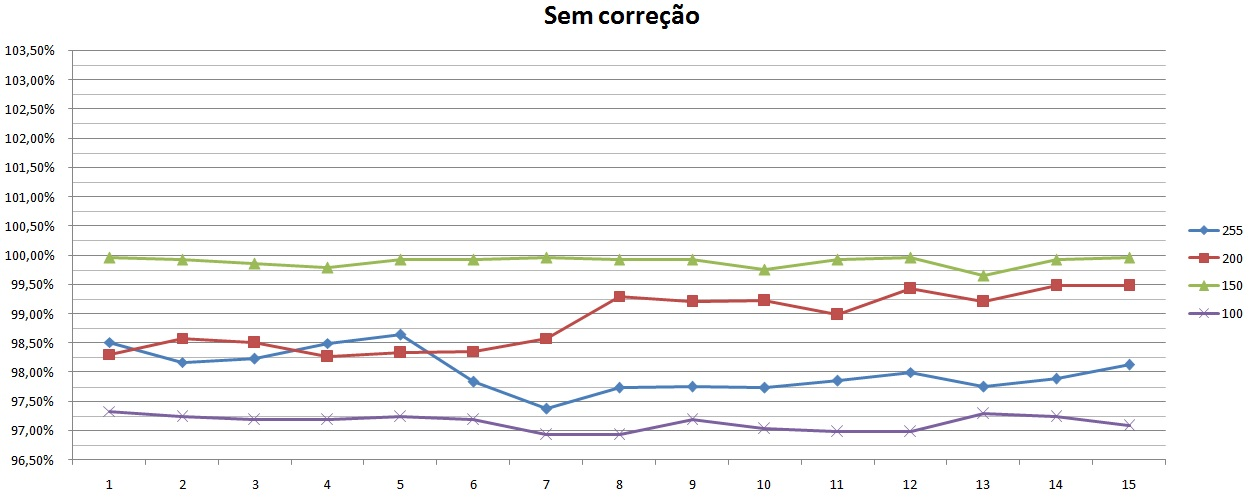
\includegraphics[width=1\textwidth]{semcorrecao.jpg}
	\caption{Velocidades do motor A em relação ao motor B em \%, quinze comparações para cada valor de PWM. Valores de PWM testados: 100, 150, 200 e 255}
	\label{fig:semcorrecao}
\end{figure}

Como pode visto no gráfico da Figura~\ref{fig:semcorrecao}, todos os valores estão abaixo de 100\%, ou seja, em todos os testes e nas quatro potências de PWM testadas. Esta diferença esta associada ao motor A permanece com uma velocidade inferior a velocidade do motor B, confirmando a necessidade de controle e também prova a diferença entre eles.

Observando esses resultados, foi proposto dois métodos para o cálculo dos pesos. O primeiro utilizando apenas o PWM mais discrepante na obtenção de amostras (PWM 100), o segundo método é a utilização dos quatro valores de PWM no momento das coletas de amostras.

\subsection{Pesos com PWM 100} \label{calib100}
Para calcular os pesos utilizando apenas como referência o PWM 100, foi utilizado a função \textbf{getAmostras(100)} quatro vezes, tendo como resultado a seguinte Tabela~\ref{Tab:calib100}.

\begin{table}[!h]
	\renewcommand{\arraystretch}{1.3}
	\centering
	\begin{tabular}{|c|cc|}
		\hline
		Amostra \# & Motor A & Motor B \\ \hline
		    1      & 127.87  & 131.93  \\
		    2      & 128.73  & 132.27  \\
		    3      & 128.80  & 132.53  \\
		    4      & 129.07  & 132.60  \\ \hline
	\end{tabular}
	\caption[Tabela de amostras PWM 100]{\small Média de quatro amostras coletadas utilizando a função \textbf{getAmostras(100)}.}
	\label{Tab:calib100}
\end{table}

Lembrando que a função \textbf{getAmostras(int \_PWM)} utiliza a função \textbf{processMedia()} ao fim de cada execução, ou seja, a função geradora de média é executada quatro vezes gerando os as médias acima apresentadas.
Ao fim das coletas passamos para o passo ao qual efetivamente calcula-se os pesos utilizando-se da função \textbf{finalMedia()}, como explicado a função determina o valor somando-se as médias de velocidade obtidas do motor A dividindo-a pelo número de amostras(quatro), somando-se as médias de velocidade do motor B e também dividindo pelo número de amostras, obtendo as duas médias do somatório das médias é realizado uma proporção com uma regra de três básica, assumindo o menor valor como o valor máximo (100\%), então obtem-se os pesos, conforme os dados do estudo o peso do motor A, representado pela variável \textbf{pesoA} com o valor de 1 (100\%) e a variável \textbf{pesoB} representando o valor do peso do motor B com o valor de 0.97 (97\%).

\begin{lstlisting}
void motorRefresh() {
	PWM_valA *= pesoA;
	PWM_valB *= pesoB;
	PWM_valA = int(PWM_valA);
	PWM_valB = int(PWM_valB);
	analogWrite(PWMA, PWM_valA);
	analogWrite(PWMB, PWM_valB);
}
\end{lstlisting}

Com os pesos determinados sempre que o programa fizer uma alteração nos valores de PWM dos motores, utilizando a função \textbf{motorRefresh()} acima descrita, este será multiplicado pelo seu respectivo peso antes de alterar efetivamente a velocidade. Sendo assim o robô calibrado com as configurações de peso acima, ao selecionar o PWM de valor 100 para ambos os motores o valor determinado para o motor A será de 100 porém o valor do motor B será de 97.

\subsection*{Resultados calibragem de unico PWM}
Ao utilizar a calibragem acima citada, a qual utiliza apenas o PWM de valor 100 na tomada de amostras para cálculo dos pesos, teve-se o seguinte resultado para os quatro PWMs (100, 150, 200 e 255).
\begin{figure}[H]	
	\centering
	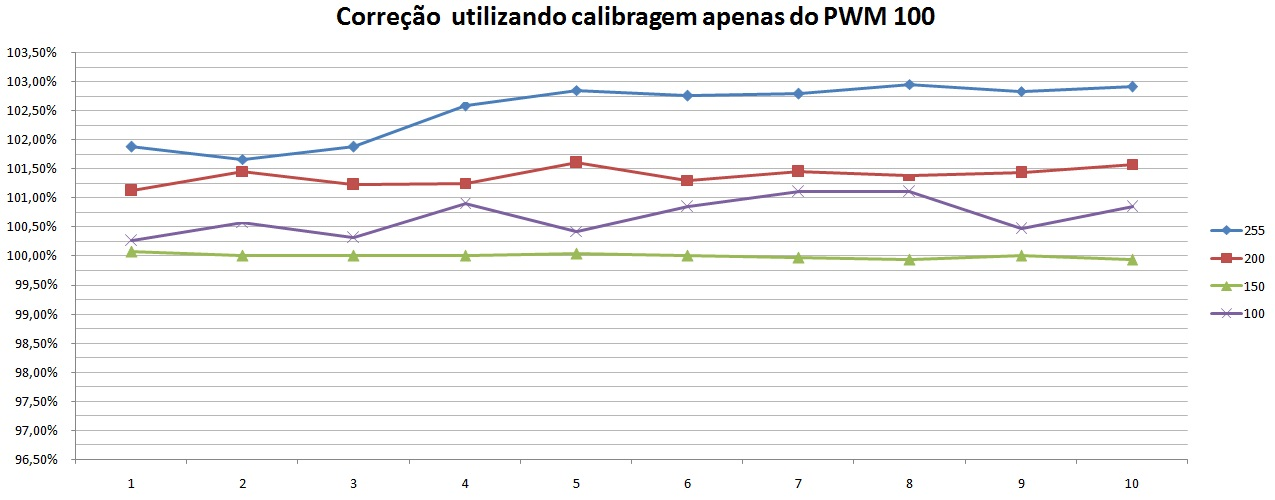
\includegraphics[width=1\textwidth]{correcao100.jpg}
	\caption{Velocidades do motor A em relação ao motor B em \%, quinze comparações para cada valor de PWM. Valores de PWM testados: 100, 150, 200 e 255}
	\label{fig:correcao100}
\end{figure}
No gráfico da Figura~\ref{fig:correcao100} podemos ver claramente que o motor A passou a ser sempre mais rápido que o moto B, com sua velocidade acima de 100\% -em relação ao motor B- para os PWM 100,200 e 255, o PWM continua estável.

\subsection{Pesos com quatro PWMs} \label{calibmult}
Afim de aumentar a precisão das correções, foi utilizado quatro valores de PWM na fase de coleta de amostras Subseção~\ref{getamostras}, tendo como resultado a seguinte Tabela~\ref{Tab:calibMC}.
\begin{table}[!h]
	\renewcommand{\arraystretch}{1.3}
	\centering
	\begin{tabular}{|c|c|cc|}
		\hline
		Amostra \# & PWM & Motor A & Motor B \\ \hline
		    1      & 255 & 347.40  & 355.33  \\
		    2      & 200 & 270.13  & 274.67  \\
		    3      & 150 & 198.87  & 202.80  \\
		    4      & 100 & 129.73  & 133.00  \\ \hline
	\end{tabular}
	\caption[Tabela de amostras PWM 100]{Tabela com a média de quatro amostras coletadas utilizando a função \textbf{getAmostras(100); getAmostras(150); getAmostras(200); getAmostras(255)}.}
	\label{Tab:calibMC}
\end{table}
Ao fim da coleta de amostras utilizou-se os quatro valores de PWM citados e finalizar a execução da função \textbf{finalMedia()} Subseção~\ref{finalMedia} tem-se os valores de 1~(100\%) para o \textbf{pesoA} e o valor de 0.98~(98\%) para o \textbf{pesoB}. Assim como citado na seção anterior os valores de PWM solicitados ao robô é multiplicado pelo seu peso antes de ser aplicado.

\subsection*{Resultado calibragem com quatro valores PWMs}
Utilizando-se da configuração acima citada a qual foi utilizado as quatro amostragens para o cálculo do peso temos o seguinte resultado.
\begin{figure}[H]	
	\centering
	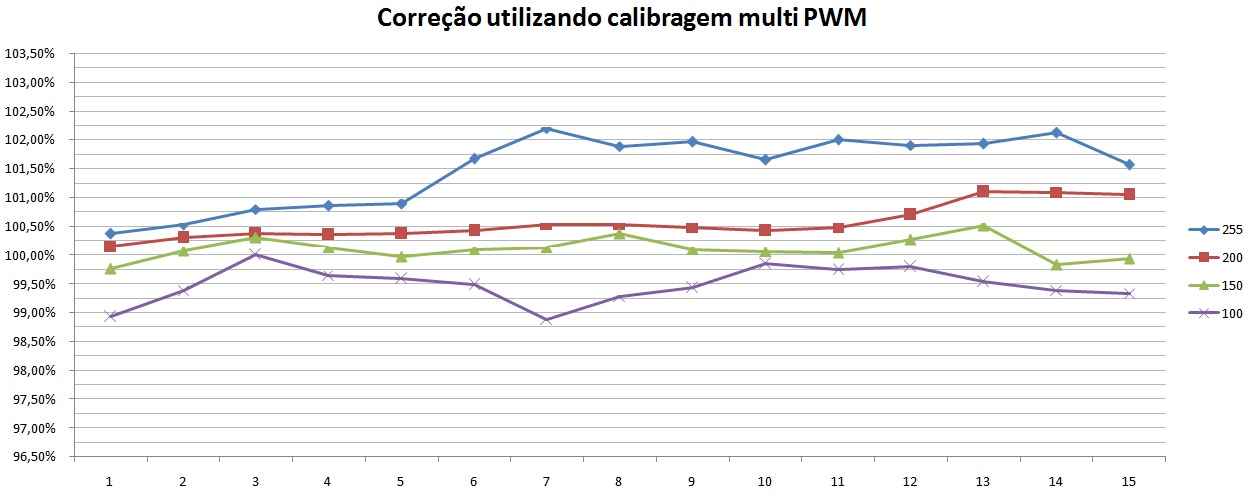
\includegraphics[width=1\textwidth]{correcao4pwm.jpg}
	\caption{Velocidades do motor A em relação ao motor B em \%, quinze comparações para cada valor de PWM. Valores de PWM testados: 100, 150, 200 e 255}
	\label{fig:correcao4pwm}
\end{figure}
Como podemos ver no gráfico acima o PWM 150 permanece mais estável que os demais valores tendo alguns testes abaixo de 100\% e outros acima. Notamos também que o robô se tornou mais equilibrado, tendo alguns valores de PWM com o motor A mais rápido e outros valores tendo o motor B como mais rápido, deixando assim o robô mais equilibrado.

\chapter{Discussão dos Resultados}
Com base nos testes realizados conforme o Capítulo~\ref{cap:desenvolvimento}, é fato que os motores necessitam de uma pequena correção para trabalharem de forma equivalente em relação as suas velocidades. 
Analisando-se o gráfico da Figura~\ref{fig:semcorrecao} confirma-se que cada PWM requer uma correção diferente, e que os regimes de grande potência (PWMs acima dos 200) se mostram menos estáveis. 

Neste capítulo utiliza-se quatro PWMs separadamente, iniciando com o PWM de valor 100.

No gráficos ilustrado pela Figura~\ref{fig:pwm100} a linha azul \textbf{(Ñ Calib $\lozenge$)} refere-se aos valores obtidos nos testes sem qualquer tipo de correção, a linha vermelha \textbf{(Mono Calib $\Box$)} aos valores obtidos nos testes utilizando apenas o PWM 100 para calibragem e por último a linha verde \textbf{(Multi Calib $\triangle$)} representando os resultados nos testes utilizando-se de quatro valores de PWM distintos (100, 150, 200 e 255) para a calibragem.

\section{Análise do PWM 100}\label{pwm100}
\begin{figure}[H]	
	\centering
	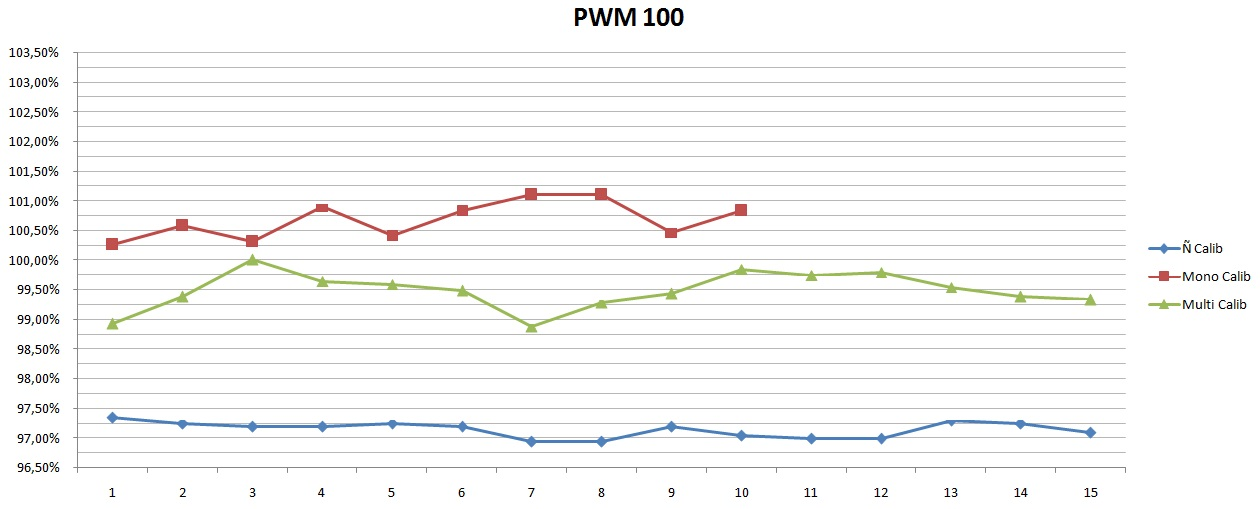
\includegraphics[width=1\textwidth]{pwm100.jpg}
	\caption{Velocidades do motor A em relação ao motor B em \%, quinze comparações para o valor de PWM 100.}
	\label{fig:pwm100}
\end{figure}

Com os dados do gráfico (Figura~\ref{fig:pwm100}) pode-se notar que o PWM 100 se mostra estável tendo em sua maior variação em apenas 1\%, comparando as amostras 1 e 3, nota-se que os resultados da calibragem utilizando um PWM, a linha vermelha, ou a calibragem com quatro valores de PWM, linha verde, se mostram eficientes, com diferença relativa de apenas 1\% para o motor A ou para o motor B, enquanto as velocidades sem correção, linha azul, apresenta uma diferença proporcional superior a 2\%.

\section{Analise do PWM 150}\label{pwm150}
\begin{figure}[H]	
	\centering
	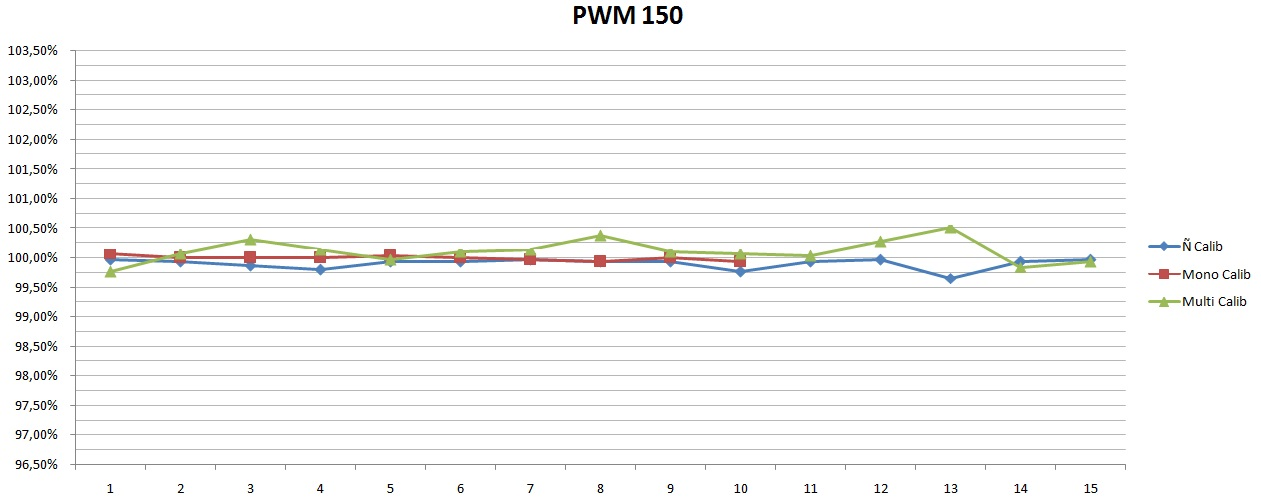
\includegraphics[width=1\textwidth]{pwm150.jpg}
	\caption{Velocidades do motor A em relação ao motor B em \%, quinze comparações para o valor de PWM 150.}
	\label{fig:pwm150}
\end{figure}

Analisando separadamente os regimes de potência pode-se notar que o valor de PWM 150 se mostra como um regime de potência mais estável. No gráfico da Figura~\ref{fig:pwm150} pode-se ver claramente que em nos três casos a diferença de velocidades dos motores não é superior a 0,5\% para mais ou para menos, tornando a correção quase desnecessária para está faixa de PWM.

\section{Analise do PWM 200}\label{pwm200}
\begin{figure}[H]	
	\centering
	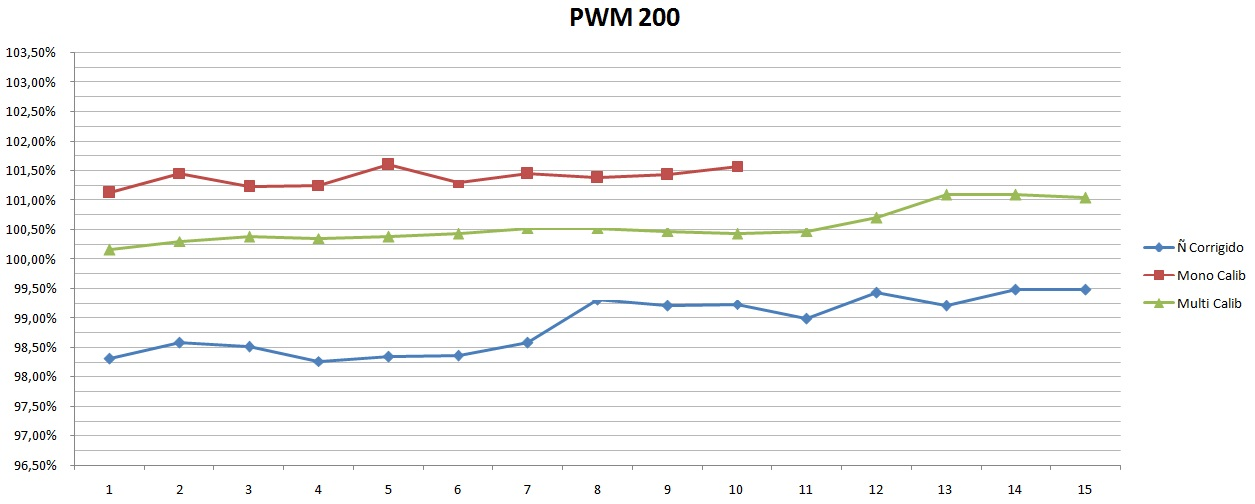
\includegraphics[width=1\textwidth]{pwm200.jpg}
	\caption{Velocidades do motor A em relação ao motor B em \%, quinze comparações para o valor de PWM 200.}
	\label{fig:pwm200}
\end{figure}
O gráfico da Figura~\ref{fig:pwm200} o qual projeta os três testes realizados com o valor de 200 para o PWM (equivalente a aproximadamente 78,43\% de toda a potência disponível) podemos notar a variação de 0,5\% ou mais entre os testes. A correção mais eficiente para este regime de potência foi o de calibragem múltipla (linha verde) conforme a Seção~\ref{fig:correcao4pwm}.

\section{Analise do PWM 255}\label{pwm255}
\begin{figure}[H]	
	\centering
	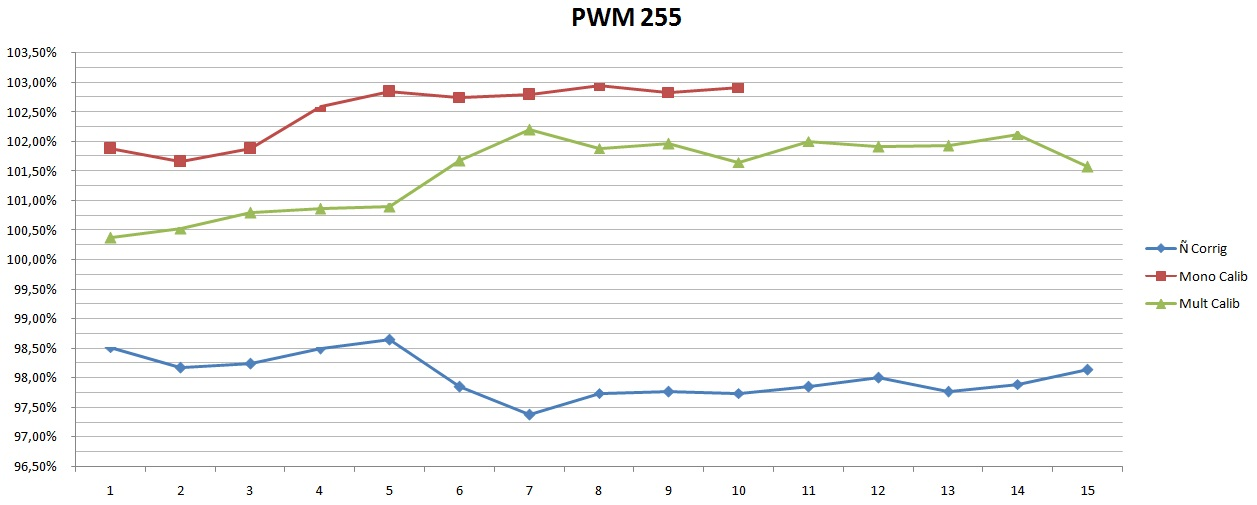
\includegraphics[width=1\textwidth]{pwm255.jpg}
	\caption{Velocidades do motor A em relação ao motor B em \%, quinze comparações para o valor de PWM 255.}
	\label{fig:pwm255}
\end{figure}

O regime de máxima potência se demonstrou o mais instável tendo variação superiores a 1\% entre as amostras no mesmo testes. Acredita-se que por se tratar da máxima potência, os motores não mantém uma consistência em seu desempenho, deixando-o mais sensível a fatores externos ou variação da corrente disponível provida pelas baterias.
Mesmo utilizando-se da calibragem com quatro valores de PWM, a qual se mostrou mais eficiente, utilizando-se destes valores de PWM ocorrem variações inesperadas. 
Tais variações -inconstâncias- podem ser notadas na Figura~\ref{fig:semcorrecao} e Figura~\ref{fig:correcao4pwm} ocorrem tanto com o valor de PWM 255 (linhas azuis $\diamond$) e com o PWM 200 (linhas vermelhas $\Box$).


%\chapter{Metodologia} \label{cap: metodologia}
%Neste trabalho foi usado apenas um sensor para cada roda -os conectados aos pinos com interrupção\ref{isr}-, sendo os sensores mais externos da roda.
%O funcionamento do encoder empregado neste trabalho é a de configuração mais simples apenas um sensor óptico, o qual realiza apenas a contagem de marcadores da fita que está colada junto a roda conforme a figura \ref{fig:roda34marc}, convertendo o movimento angular das rodas em sinais digitais, estes sinais são utilizados como sinais de entrada para as interrupções \ref{isr}, realizando a contagem do número de pulsos em determinado tempo.

%\begin{enumerate}[(A)]
	
%	\item Desenvolvimento e entrega do plano de trabalho;
%	\item Escrita da introdução, levantamentos dos dados teóricos e bibliográficos.
%	\item Revisão da literatura. 
%	\item Implementar a aplicação
%	\item Escritas do trabalho de conclusão do curso.		
	
%\end{enumerate}

\chapter{Considerações Finais}
Um dos principais problemas da robótica móvel esta em como controlar a trajetória de forma precisa. A equipe Cedro/CPCX de futebol de robôs, participante da categoria VSS-RoboCup, tem enfrentado este problema pois os robôs Modu não andam em linha reta quando aplicado o mesmo PWM para ambos os motores.

Primeiramente foi estudado, implementado e testado, um sistema embarcado de controle tipo PID. Contudo foram identificados problemas de coerência  dos dados coletados. Posteriormente, foi verificado que estes problemas estavam diretamente relacionados ao conflito de interrupções e a forma com a qual o Atmega trata as ISRs.

Com um estudo aprofundado das interrupções do Atmega328 foi identificado primeiramente a lista das prioridades de interrupção.
Além disso, foi constatado que durante o atendimento de uma ISR as demais interrupções são ignoradas. Portanto, não é possível coletar simultaneamente as interrupções de ambas as rodas, pois devido ao grande número de interrupções, muitas dessas serão ignoradas, causando erro no ajuste do tipo PID.

Considerando o modelo de tratamento de interrupções do Atmega328, foi proposto um sistema embarcado que atua como uma ferramenta para monitoramento e ajuste individual da velocidade das rodas. 
%
Neste sistema utiliza-se das médias das contagens de interrupções para determinar a diferença relativa da velocidade entre os motores. 
Utilizando-se de uma sintaxe própria, criada durante o desenvolvimento deste trabalho, é possível tornar o sistema uma ferramenta capaz de testar, monitorar e ajustar regimes de potência para um ou mais PWMs.

Por fim observou-se por meio dos testes, a necessidade de diferentes ajustes para diferentes regimes de potência e que a ferramenta se mostrou eficaz como pré-ajuste do peso, para uma determinada velocidade, conforme a necessidade da competição.


\section*{Principais contribuições}
A principais contribuições deste trabalho foram:
\begin{itemize}
	\item Ferramenta de monitoramento das velocidades dos motores, com a qual pode-se verificar quais valores são mais estáveis de PWM para serem utilizados em competições;
	\item Definição da sintaxe de comunicação para controle do robô, bem como, monitoramento e ajuste do peso dos motores;
	\item Estudo do comportamento das interrupções no Atmega328;
	\item Estudo e implementação do PID, e constatação da não possibilidade de correção das velocidades em tempo real com a arquitetura do Arduino Nano.
\end{itemize}


\section*{Trabalhos Futuros}
Como sugestão de trabalhos futuros, propõe-se:
\begin{itemize}
	\item Alterar a função de calibragem a fim de gerar uma tabela com N faixas de PWMs e determinar um peso ideal para cada faixa.
	\item Dar a capacidade do sistema determinar uma nota de 0 a 10 que messa a equidade dos motores.
	\item Determinar quais os valores de PWM mais estáveis e sugerir não utilização dos mais instáveis.
\end{itemize}


\cleardoublepage
%\phantomsection
\addcontentsline{toc}{chapter}{Referências Bibliográficas} 
\bibliographystyle{abnt-alf}
%\bibliographystyle{apalike} 
%\bibliographystyle{ieeetr} % Ordena por ordem de aparição.  
%\bibliographystyle{abbr} % Ordena por ordem alfabetica com nomes abreviados.
%\bibliographystyle{plain} % Ordena por ordem alfabetica com nomes por extenso.
\bibliography{bibliografia} % commented if *.bbl file included.

%\addcontentsline{toc}{chapter}{Ap\^endices}
\appendix
\chapter{Joystick Bluetooth}
Um simples projeto foi desenvolvido também em Arduino. O projeto tem a finalidade de ser um controle bluetooth com um Joystick, utilizado para controlar as direções do robô. 
O joystick, um dos componentes do controle, nada mais é que dois potenciômetros, um potenciômetro para os valores do eixo X e outro para os valores do eixo Y. 
O controle possui um componente bluetooth para estabelecer uma troca de dados junto ao robô, o qual também possui seu componente bluetooth, o qual será explicado no Seção~\ref{bthc06}.
O código atualizado pode ser encontrado no link: https://github.com/kelvimro/TCCTerceira/blob/master/lib/ ControleBT/controleBT.cpp 
O controle tem o intuito de simular os comandos que são gerados pela inteligência artificial no software que é responsável pelas táticas e movimento dos jogadores durante uma partida.
Os comandos podem variam entre -100 até 100, tendo um valor para cada motor, ou seja cada computação realizada pela inteligência artificial é enviado dois números inteiros, onde o primeiro número é destinado ao motor esquerdo e o segundo ao direito.
Utilizando-se da função map() a qual proporciona os valores do potenciômetro - dos quais variam entre 0 a 1023 - aos valores válidos para o robô.

\begin{lstlisting}
if (cmdX >= 0 && cmdX <= 501) cmdX = map(cmdX, 0, 501, -100, 0);
else cmdX = map(cmdX, 502, 1023, 0, 100);
if (cmdY >= 0 && cmdY <= 509) cmdY = map(cmdY, 0, 509, -100, 0);
else cmdY = map(cmdY, 510, 1023, 0, 100);
\end{lstlisting}

O potenciômetros Y, o qual vai representar os valores de potência, em posição neutra (sem ação do controlador) encontra-se com valor analógico de 509, então mapeado para 0, ou seja, não há potência requerida.
Ao movimentar o joystick para frente, aumenta-se o valor analogio do potenciômetro até o máximo de 1023 que após ter seu valor mapeado representa o valor 100.
Movimentando o joystick para trás, os valores analógicos lido diminuem até 0, denotando o valor -100. 
\\
\begin{lstlisting}
if (cmdY >= 0 && cmdY <= 509) cmdY = map(cmdY, 0, 509, -100, 0);
else cmdY = map(cmdY, 510, 1023, 0, 100);
\end{lstlisting}

Valores positivos no eixo Y indicam que o movimento solicitado é para frente, enquanto os valores negativos representam movimento para trás.
O potenciômetros X, o qual vai representar os valores da diferença entre os motores. Em sua posição neutra tem o valor analógico lido de 502, representando 0\% de diferença entre os motores. Afim de facilitar a compreensão chamaremos de A o motor do lado esquerdo e de B o motor do lado direito. Então ao movimentar o joystick para a esquerda o valor analógico lido diminui até 0, resultando no valor de -100, movimentando o joystick para a direita aumentando o valor analógico lido até 1023 que representa o valor 100. 
\begin{lstlisting}
if (cmdX >= 0 && cmdX <= 501) cmdX = map(cmdX, 0, 501, -100, 0);
else cmdX = map(cmdX, 502, 1023, 0, 100);
\end{lstlisting}
No eixo X os valores negativos indicam que o motor A tem de se movimentar X\% mais lento em relação ao motor B, fazendo o movimento de curva para o lado de A. Já com os valores positivos de X indica que o motor B deve ser X\% mais lento q o A fazendo a curva para o lado B.

\chapter{getAmostras(int \_PWM)}\label{anexo:getamostra}
\begin{lstlisting}
void getAmostras(int _PWM) {
print = "PWM =\t";
print += _PWM;
// https://www.arduino.cc/en/Reference/NoInterrupts
noInterrupts();									// Desativa interrupções
print += "\nA:\n";
PWM_valA = _PWM;				// PWM_valA é o PWM do motor A de 0 a 255
PWM_valB = 1;					// PWM_valA é o PWM do motor A de 0 a 255
motorRefresh();
countB = countA = 0;
static double calibMillis;				   	// calibMillis timer de loop
calibMillis = millis();
interrupts();									// Reativa intrrupções
while (PWM_valA >= 5) {
for (int i = 0; i < NUM_AMOSTRA; ++i) {// Controla numero de amostras
// Enquanto encoder conta durante CALIBMILLIS, faça nada ;)
while ((millis() - calibMillis) <= CALIBMILLIS) {}
noInterrupts();         				   // Desarma interrupts
calibA.push(countA);// Adiciona a ultima contagem a fila de amostras
print += countA;
print += "\n";
countA = 0;                  // Zera contadores de marcos do encoder
calibMillis = millis();				    // Zera o contador de tempo
interrupts();              						// Arma interrupsts
}
PWM_valA = PWM_valB = 2;				// Reduz vel. mas mantem sentido
motorRefresh();
}
noInterrupts();										// Desativa interrupções
// Set PWM - config inicial
print += "\nB:\n";
PWM_valA = 1;
PWM_valB = _PWM; 			 	   // PWM_valA é o PWM do motor A de 0 a 255
motorRefresh();
countB = countA = 0;
calibMillis = millis();
interrupts();
while (PWM_valB >= 5) {
for (int i = 0; i < NUM_AMOSTRA; ++i) {
// Enquanto conta durante CALIBMILLIS, faça nada :)
while ((millis() - calibMillis) <= CALIBMILLIS) {}
noInterrupts();								 // Desarma interrupts
calibB.push(countB);
print += countB;
print += "\n";
countB = 0;				 	// Zera contadores de marcos do encoder
calibMillis = millis();
interrupts();									// Arma interrupsts
}
PWM_valA = PWM_valB = 2;
motorRefresh();
}
Serial.print(print); 	   			// Imprime o conteudo da variavel print
print = " ";			 							// Esvazia variavel print
if (processMedia()) {}    // Invoca o metodo responsavel por calcular a média
}
\end{lstlisting}

Como pode ser visto no código acima, na linha 1 encontra-se a declaração do método do tipo \textit{void} (sem retorno). Excluindo as linhas da variável \textit{print} da explicação visto que a mesma é utilizado apenas para armazenar os dados a serem exibidos para o úsuario, pode-se observar nas linhas 5, 18, 29 e 42 a presença da função \textbf{noInterrupts();} e nas linhas 13, 24, 37 e 48 a função \textbf{interrupts();} ambos explicados na Seção~\ref{usointerrupcao}. 
As linhas 12, 23, 36 e 47 contém a função \textbf{millis();} a qual retorna um número referente ao tempo em que o Arduino encontra-se ligado, sendo assim nas linhas citadas, é armazenado o ``horário" da execução naquele instante e gravado na variável \textbf{calibMillis}.
Os PWMs são utilizados como critérios de parada nos laços \textit{while} nas linhas 14 e 38, sendo alterados apenas quando o laço \textit{for} da linha 15 obter o número de amostras determinado em \textbf{NUM\_AMOSTRA}.
As duas estruturas de repetição \textit{while}, nas linhas 17 e 41 utiliza-dos como espera, a fim de evitar o uso da função \textbf{delay();} a qual utiliza-se de interrupções.
Sendo assim não há execução de nenhum código até que o tempo atual obtido por meio da função \textbf{millis()} subtraindo o ``horário da ultima execução -armazenado na linha 12- seja maior que o tempo de coleta determinado na variável \textbf{CALIBMILLIS}, após decorrido intervalo determinado na variável \textbf{CALIBMILLIS}, é desativado as interrupções conforme a linha 18 a fim de não aumentar a contagem de marcadores.
A contagem de interrupções é armazenada na variável \textbf{contA}, este valor é então adicionado a uma estrutura de fila declarada como \textbf{calibA}, conforme a linha 19 logo então é armazenada a última contagem este contador é zerado na linha 22, anotando-se o tempo atual conforme a linha linha 23 e reativando as interrupções na linha 24.
Este processo será executado até obter o número desejado de amostras devido a função \textit{for} da linha 15, ao fim, obtendo o número total de amostras os PWMs do motor A e B são setados para 2, a fim de para-los, então chamado o método \textbf{motorRefresh();} o qual atualiza os valores de PWM nos motores como pode ser visto no código abaixo, finalizando então a coleta de amostras para o motor A.

\begin{lstlisting}
void motorRefresh() {
PWM_valA *= pesoA;
PWM_valB *= pesoB;
PWM_valA = int(PWM_valA);
PWM_valB = int(PWM_valB);
analogWrite(PWMA, PWM_valA);
analogWrite(PWMB, PWM_valB);
}
\end{lstlisting}

O mesmo processo ocorre para aquisição de amostras para o motor B entre as linhas 29 e 52, desativando interrupções, determinando o valor do PWM de B para o PWM a ser testado, zerando os contadores, armazenando o tempo atual, fazendo as esperas utilizando-se da estrutura \textit{while} assim como ocorreu no motor A.

\chapter{processMedia()} \label{anexo:processmedia}

\begin{lstlisting}
boolean processMedia() {
static double _soma;
_soma = 0;
static double _med;
_med = 0;
static int _mark;
_mark = 0;
print = "\nMédia\t";
while (!calibA.isEmpty()) {
_soma += calibA.pop();
_mark++;
}
_med = _soma / _mark;
mediaA.push(_med);
print += _med;                   			         // Imprime média de A
_soma = 0;
_med = 0;
_mark = 0;
while (!calibB.isEmpty()) {
_soma += calibB.pop();
_mark++;
}
_med = _soma / _mark;
mediaB.push(_med);
print += "\t";         			       // Imprime indicadores e média de B
print += _med;
delayMicroseconds(999);
Serial.println(print);	
return true;
}	
\end{lstlisting}

A função começa declarando três variáveis locais (\textbf{\_soma, \_med e \_mark}), pois são utilizadas apenas dentro da função, estas variáveis são utilizadas para auxiliar nos cálculos. 
Declaradas como estáticas afim de economizar memória, utiliza-se a mesma variável sempre que a função for chamada. 
Ao instanciar as variáveis nas linhas 2, 4 e 6 e zeradas nas linhas 3, 5 e 7 inicia-se o processo de cálculo da média propriamente dita, na linha 9 onde encontra-se o critério de parada da estrutura de repetição \textit{while}, critério este o resultado da função \textit{.isEmpty()}, uma função disponível na estrutura de dados da variável \textbf{calibA} e \textbf{cablibB} que são do tipo fila (\textit{array}), esta função -\textit{.isEmpty()}- retorna verdadeiro (\textit{true}) caso a fila esteja vazia, sendo assim enquanto a fila \textbf{calibA} não estiver vazia soma-se o atual valor de \textbf{\_soma} ao valor retirado da fila, utilizando a função \textit{.pop()} conforme a linha 10, então incrementando 1 o valor de \textbf{\_mark} na linha 11, a variável \textit{\_mark} tem por finalidade contar o número exato de amostras retiradas da fila, ou seja, sempre uma amostra for retirada da fila é incrementado em um ao marcador. Assim que todos as amostras forem retiradas da fila e somadas a variável responsável por armazenar temporariamente o valor da média a variável \textbf{\_med} recebe a divisão da \textbf{\_soma} pelo \textbf{\_mark}, o número de elementos contados, tendo então a média das amostras obtidas, com o valor computado em mãos este é inserido em outra fila chamada de \textbf{mediaA} por meio da função \textit{.push()} passando \textbf{\_med} como argumento, conforme a linha 14. Ao finalizar o cálculo da média das amostras do motor A o mesmo ocorre com as amostras do motor B, para isso inicia-se zerando as três variáveis auxiliares locais nas linhas 16, 17 e 18, passando pelo mesmo processo de retirada da fila, soma, divisão e adicionando a pilha de médias de B, como pode ser visto entre as linhas 19 e 24 tendo como diferença apenas as variáveis responsáveis para o cálculo do motor B.

\chapter{Função de teste - getPercent()}\label{getPercent}
A função de teste é muito similar a função \textbf{finalMedia()} tendo apenas duas diferenças básicas. A primeira diferença é a divisão não será a menor velocidade dividido pela maior e sim a velocidade do motor A dividido pela velocidade do motor B, sendo assim, sempre será calculado a proporcionalidade da velocidade do motor A em relação a velocidade do motor B, imprimindo seu valor proporcional em percentagem(\%), tendo um valor superior a 100\% quando a velocidade do motor A for mais rápida que a velocidade do motor B e inferior a 100\% quando a velocidade menor.
A segunda diferença é que o resultado dos cálculos são apenas apresentados para o estudo das diferenças, ou seja, os valores não são salvos nas variáveis de peso e sim salvas nas variáveis locais e temporárias \textbf{\_pA} e \textbf{\_pB}.
\begin{lstlisting}
boolean getPercent() {
static double _soma;
_soma = 0;
static double _med;
_med = 0;
static int _mark;
_mark = 0;
while (!mediaA.isEmpty()) {
_soma += mediaA.pop();
_mark++;
}
_med = _soma / _mark;
static double _pA;
_pA = _med;
_soma = _med = 0;
_mark = 0;
while (!mediaB.isEmpty()) {
_soma += mediaB.pop();
_mark++;
}
_med = _soma / _mark;
static double _pB;
_pB = _med;
delayMicroseconds(2000);
print = "\nPerc\t";
print += ((_pA / _pB) * 100);
print += "%";
Serial.println(print);
}
\end{lstlisting}
Conforme visto acima, a função não altera nenhuma variável com influência nas configurações dos motores, apresentando apenas uma proporção entre os motores.


%\include{apendice}

\end{document}